\documentclass{book}

\usepackage{graphicx} % Images
\usepackage{listings} % Code snippets
\usepackage{placeins} % \FloatBarrier
\usepackage[skip=10pt]{parskip} % Para spacing

\title{The Cg Tutorial}
\author{Randima Fernando, Mark J. Kilgard}
\date{2003}

\begin{document}
\frontmatter

\maketitle

\tableofcontents
\listoffigures
\listoftables

\mainmatter

\chapter*{Foreword}

Real-time computer graphics hardware is undergoing a major transition, from supporting a few fixed algorithms to being fully programmable. At the same time, the performance of graphics processors (GPUs) is increasing at a rapid rate—even greater than that of CPUs—because GPUs can effectively exploit the enormous parallelism available in graphics computations. These improvements in GPU flexibility and performance are likely to continue in the future, and will allow developers to write increasingly sophisticated and diverse programs that execute on the GPU.

Until recently, most GPU programs were written in assembly language, but history has shown that developers make the most creative and effective use of programmable hardware when they have the opportunity to program in a high-level language. Our goal in designing Cg was to provide developers with the same flexibility and performance available in assembly language, but with the expressiveness and ease-of-use of a high-level language. The C language has demonstrated enormous success in achieving these goals on the CPU, and so we chose C's syntax and philosophy as the starting point for defining Cg. In particular, this choice gave us confidence that the Cg language would be able to implement any GPU program, rather than restricting developers to a predefined framework designed specifically for shading computations.

Cg also builds on ideas and lessons learned from earlier work in computer graphics. My personal interest in programmable graphics hardware was inspired by the PixelFlow project at the University of North Carolina and, in particular, by the shading language compiler that Marc Olano and others built for PixelFlow. In many respects, the most direct predecessor to Cg was the real-time programmable shading system that Kekoa Proudfoot, Pat Hanrahan, I, and others built at Stanford for single-chip GPUs. The knowledge that we acquired from building the Stanford system was crucial to the design of Cg. Offline movie rendering has relied on programmable shading for much longer. The RenderMan language designed by Pat Hanrahan at Pixar served as a major source of inspiration for Cg, particularly in the choice of Cg's built-in functions.

The desire to create one GPU programming language that would be widely supported for both the OpenGL and Direct3D APIs led us to collaborate with Microsoft on the design of Cg. Microsoft's implementation of the language is called HLSL, and it is shipped as part of DirectX 9. At Microsoft, Craig Peeper and Loren McQuade were particularly influential in the design of the language. The examples in this book work equally well with HLSL and Cg.

Designing and implementing Cg in less than a year was possible only because we had a large and highly talented team of people working together. Two individuals made particularly unique contributions. Steve Glanville's extensive compiler and language expertise was crucial to the Cg design effort, and he implemented most of the front end of the first version of the Cg compiler. Kurt Akeley's experience as a system designer was invaluable throughout the project.

In this book, Randy and Mark have assembled a series of Cg tutorials that introduce Cg while simultaneously describing many of the real-time shading techniques supported by modern GPUs. By integrating these two sets of concepts within one collection of tutorials, this book enables you to experience the fun of writing and experimenting with your own GPU programs. Enjoy the journey!

Bill Mark

Cg Language Lead Designer

Assistant Professor

The University of Texas at Austin

\chapter*{Preface}

Once upon a time, real-time computer graphics was all about vertices, triangles, and pixels. In fact, it still is. However, the level at which a programmer controls the processing and appearance of these graphics primitives has advanced considerably. Until a few years ago, programmers had to rely on the CPU to process all the transformation and rasterization algorithms needed to produce computer-generated images. Over time, hardware engineers executed these algorithms via specialized, high-performance 3D graphics hardware. Rather than implement the algorithms directly, programmers learned to access the hardware-provided graphics functionality through standard 3D programming interfaces, such as OpenGL (developed by Silicon Graphics [SGI]) and Direct3D (developed by Microsoft). At first, such costly 3D graphics hardware appeared only in high-priced UNIX workstations and flight simulators. Now, through the miracle of Moore's Law, the benefits of graphics hardware acceleration have been bestowed on low-cost PCs and game consoles.

Although the performance gained by employing dedicated graphics hardware to execute the brute-force tasks of transforming vertices, rasterizing triangles, and updating pixels far exceeded the performance possible just with CPU programming, real-time 3D programmers gave up a considerable measure of control in exchange for this speed. Developers were limited to using a fixed-function palette of graphics operations that the hardware could handle. Sometimes a skilled and dedicated programmer could coax the graphics programming interface and hardware to accomplish something beyond the ordinary, but this was usually hard, time-consuming work.

While graphics hardware engineers were advancing the real-time performance of their specialized pixel-pushing hardware, off-line computer graphics software packages such as Pixar's PhotoRealistic RenderMan were changing the look of movies and television with amazing computer-generated special effects. The pre-recorded nature of movies and most television content makes these media well suited for offline rendering. Computer-generated images for film and video are not rendered in real time but instead carefully constructed frame by frame in hours, days, or weeks using standard general-purpose CPUs. The advantage of using general-purpose CPUs is that rather than settle for hard-wired hardware algorithms, programmers and artists can use the CPU to create any effect they might imagine. What these so-called offline rendering systems lack in relative speed, they make up in rendering quality and realism.

The flexibility and generality of offline rendering systems are the key features that have been missing from preceding generations of 3D graphics hardware. In other words, what was lost was programmability.

Realizing this limitation, computer graphics architects have designed a new generation of graphics hardware that permits an unprecedented degree of programmability. Now, many of the programmable shading techniques that are employed so successfully in offline rendering can enter the realm of real-time graphics.

Developers of offline rendering systems created a type of specialized computer language known as a shading language to express the graphics operations required to make surfaces look the way artists intend. A shading language for programmable graphics hardware provides the same sort of functionality but in the context of real-time graphics hardware. Graphics programmers and artists benefit from such a high-level programming language in much the same way that conventional programmers do from C++ or Java. Using a high-level language for graphics hardware automates the process of translating the programmer's intent into a form that the graphics hardware can execute.

This book is about Cg, the premier language for programmable graphics hardware. NVIDIA developed Cg in close collaboration with Microsoft. Cg is the most portable and productive way for you to unleash the power within programmable graphics hardware. This book is a tutorial to teach you how to write Cg programs.

\section*{Our Intended Audience}

We tried to write this book in a way that makes it valuable to both novices and advanced readers. If you're new to the world of programmable graphics, this book should give you a firm foundation on which to build. If you encounter a word or concept that is foreign to you and not sufficiently explained, consult the "Further Reading" section at the end of each chapter.

The main audience for this book is 3D game and application programmers, managers of such projects, real-time 3D artists, and computer graphics students—or anyone else interested in learning about the state of the art in real-time rendering. You do not have to be an experienced programmer to learn Cg from this book, though you should be relatively familiar with programming language concepts. If you are familiar with C or one of its derivatives, such as C++ or Java, Cg will be very approachable. Cg programs are relatively short, often less than a page, so even an artist or novice programmer can get the gist of Cg from this tutorial and learn to write interesting Cg programs.

Computer graphics programming involves math. Understanding basic algebra and trigonometry will help you appreciate several sections. You should also be familiar with the math behind basic computer graphics vertex transformation and lighting models. You do not need to know OpenGL or Direct3D, but familiarity with either programming interface is very helpful. All of the Cg examples described work with either OpenGL or Direct3D unless otherwise noted. Some examples that require advanced Cg functionality may not work on older graphics processors.

\section*{The Book's Structure}

Chapter 1 introduces Cg. Each chapter that follows is a short tutorial that presents specific Cg concepts and techniques. The tutorials build upon each other, so we recommend reading the chapters in order.

\FloatBarrier
\begin{itemize}
\item Chapter 1 lays out the foundations of Cg and real-time programmable graphics hardware.
\item Chapter 2 presents the simplest Cg programs.
\item Chapter 3 explains parameters, textures, and expressions.
\item Chapter 4 shows how to transform vertices.
\item Chapter 5 covers the implementation of lighting models with Cg.
\item Chapter 6 describes how to animate and morph models with Cg vertex programs.
\item Chapter 7 explains environment mapping with Cg.
\item Chapter 8 shows how to implement bump mapping.
\item Chapter 9 discusses a number of advanced topics: fog, cartoon shading, projected spotlights, shadow mapping, and compositing.
\item Chapter 10 explains the set of currently available Cg vertex and fragment profiles, and provides advice for improving the performance of Cg programs.
\end{itemize}
\FloatBarrier

This book gets you started but does not contain everything you will eventually want to know about Cg. This tutorial complements other documentation (such as the Cg Toolkit User's Manual: A Developer's Guide to Programmable Graphics) included with the Cg Toolkit. Please consult the user's manual and other Cg documentation for further information.

\section*{Formatting Conventions}

Various elements in this book are specially formatted for easier reading. Code samples are written in the Courier font on a light reverse highlight. Variables and keywords are in \textbf{bold Courier} in the text, and key concepts are \textit{italicized}.

In addition, we use icons to identify special topics, as shown here.

\textbf{Advanced Topic.} Provides extra insight for advanced readers but can be safely glossed over without loss of continuity.

\textbf{Caution.} Indicates a subtlety or concept to be wary of when writing Cg code, to avoid errors.

\textbf{CineFX.} Describes algorithms or features that are available only on the NVIDIA CineFX architecture, or on architectures with similar advanced capabilities.

\textbf{Coding Tip.} Gives guidelines about good coding practices.

\textbf{Performance Tip.} Points out ways to use Cg to achieve optimal GPU performance.

\section*{Trying the Examples}

We've designed the accompanying software framework so that you can get straight to work, even if you don't know anything about OpenGL, Direct3D, C, or C++. Our goal is to isolate the Cg language and allow you to experiment freely with it. Of course, as you move toward starting a real-world application with Cg, your project will probably require some combination of OpenGL, Direct3D, C, and C++.

The accompanying software framework allows you to try out the various Cg examples in the book without worrying about graphics APIs, C, or C++ code. The latest versions of the applications are free to download via the book's companion Web site. The software on the accompanying CD works only on the Windows platform, but versions for Linux and Macintosh systems are available online. Appendix A explains how to download the latest versions of Cg and the accompanying tutorial application.

The tutorial application makes it easy for you to tweak the book's examples, to see how changing a particular Cg example can immediately affect the rendered 3D result. If you can, have a computer that supports Cg nearby to try out the examples. With our software, you just write Cg programs without worrying about the particulars, such as loading 3D models and textures. When you want to know all the gory details, examine the source code, all of which is freely available for download, so you can see how Cg interfaces with C++ and OpenGL or Direct3D. The Cg Toolkit also comes with several simple examples that you can learn from.

The end of each chapter includes suggested exercises that you can work on to explore Cg further.

\section*{Acknowledgments}

We would like to thank our many colleagues at NVIDIA who contributed to Cg and helped us with this book. Bill Mark, Steve Glanville, Mark Kilgard, and Kurt Akeley worked to define the original Cg language in 2001 and 2002. David Kirk, Jensen Huang, Dwight Diercks, Matt Papakipos, and Nick Triantos recognized the need for a high-level language for graphics processors and provided the resources necessary to make Cg a priority and a reality in just over a year's time. Geoff Berry, Michael Bunnell, Chris Dodd, Cass Everitt, Wes Hunt, Craig Kolb, Jayant Kolhe, Rev Lebaredian, Nathan Paymer, Matt Pharr, Doug Rogers, and Chris Wynn developed the Cg compiler, Standard Library, and runtime technology. Sim Dietrich, Ashu Rege, and Sébastien Dominé worked on the original CgFX technology. Chris Seitz gave us a great deal of support in all aspects of the project, helping out in ways that are too numerous to list, but without which this book would not exist. John Spitzer provided the clear foresight, as well as the essential resources, for Cg's development, and gave us the backing from his team to make this book possible. Sanford Russell's contagious motivation helped to get this book started. Cyril Zeller created the handy tutorial framework that accompanies this book and contributed the material for Appendix B. Sim Dietrich shared his knowledge of CgFX in Appendix C. Kevin Bjorke lent his insight by writing the compositing section of the advanced chapter. Teresa Saffaie, Catherine Kilkenny, and Debra Valentine reviewed our writing in an effort to make it clear. Caroline Lie, Spender Yuen, Dana Chan, Huey Nguyen, and Steve Burke lent their creativity and imagination to design and beautify the book's cover, figures, and artwork. NVIDIA's demo team (Curtis Beeson, Dan Burke, Joe Demers, Eugene d'Eon, Steve Giesler, Simon Green, Daniel Hornick, Gary King, Dean Lupini, Hubert Nguyen, Bonnie O'Clair, Alexei Sakhartchouk, and Thant Tessman, under the direction of Mark Daly) contributed several of the color plates.

We are also grateful to Jason Allen, Geoff Berry, Michael Bunnell, Sim Dietrich, Chris Dodd, Gihani Fernando, Simon Green, Larry Gritz, Eric Haines, Wes Hunt, Gary King, Craig Kolb, Jayant Kolhe, Eric Lengyel, Cameron Lewis, Gilliard Lopes, Viet-Tam Luu, Kurt Miller, Tomas Akenine-Möller, Russell Pflughaupt, Matt Pharr, John Spitzer, Nick Triantos, Eric Werness, Matthias Wloka, Cyril Zeller, and our anonymous reviewers for their invaluable comments in the review process. Each set of comments helped to make the book clearer and more accurate.

Microsoft and NVIDIA collaborated to agree on the syntax and semantics of a standard hardware shading language. The DirectX 9 High-Level Shading Language and Cg are the same language because of this effort. We particularly appreciate the work of Craig Peeper, Loren McQuade, Dave Aronson, Anuj Gosalia, Chas Boyd, and Mike Toelle.

We acknowledge the pioneering research on hardware shading languages conducted at the University of North Carolina and Stanford University. Obviously, Pixar's RenderMan Shading Language provided a great deal of inspiration for NVIDIA's efforts to develop a real-time language for mass-market graphics hardware. Ken Perlin's work on the Pixel Stream Editor, not to mention his early Cg compiler testing, deserves recognition as well.

On the hardware front, we acknowledge the fundamental work of Erik Lindholm and Henry Moreton, who architected the user-programmable vertex processing engine inside NVIDIA's GeForce3 GPU. OpenGL's and Direct3D's support for general programmable vertex processing, and hence Cg's support for the same, are indebted to this work.

The hard work and dedication of NVIDIA's architecture, hardware, and software engineers to deliver ever faster and ever more programmable graphics processors was and still is the overriding justification for Cg. We acknowledge the efforts of all the engineers at NVIDIA who strive to make real-time programmable shading a reality for everyone.

We thank the Addison-Wesley production team for making this book a reality. We particularly thank Chris Keane for manhandling our manuscript into shape.

Finally, we thank the thousands of Cg developers for their feedback, bug reports, patience, and enthusiasm.

\chapter{Introduction}

This chapter has the following four sections:

\FloatBarrier
\begin{itemize}
\item "What Is Cg?" introduces the Cg programming language.
\item "Vertices, Fragments, and the Graphics Pipeline" describes the data flow of modern graphics hardware and explains how Cg fits into this data flow.
\item "Cg's Historical Development" provides some background on how Cg was developed.
\item "The Cg Environment" explains how applications go about using Cg programs through the Cg runtime and existing 3D application programming interfaces (APIs).
\end{itemize}
\FloatBarrier

\section{What Is Cg?}

This book teaches you how to use a programming language called Cg. The Cg language makes it possible for you to control the shape, appearance, and motion of objects drawn using programmable graphics hardware. It marries programmatic control of these attributes with the incredible speed and capabilities of today's graphics processors. Never before have computer graphics practitioners, whether artists or programmers, had so much control over the real-time images they generate.

Cg provides developers with a complete programming platform that is easy to use and enables the fast creation of special effects and real-time cinematic-quality experiences on multiple platforms. By providing a new level of abstraction, Cg removes the need for developers to program directly to the graphics hardware assembly language, and thereby more easily target OpenGL, DirectX, Windows, Linux, Macintosh OS X, and console platforms such as the Xbox. Cg was developed in close collaboration with Microsoft Corporation and is compatible with both the OpenGL API and Microsoft's High-Level Shading Language (HLSL) for DirectX 9.0.

Cg stands for "C for graphics." The C programming language is a popular, general-purpose language invented in the 1970s. Because of its popularity and clean design, C provided the basis for several subsequent programming languages. For example, C++ and Java base their syntax and structure largely on C. The Cg language bases itself on C as well. If you are familiar with C or one of the many languages derived from C, then Cg will be easy to learn.

On the other hand, if you are not familiar with C or even programming languages in general but you enjoy computer graphics and want to learn something new, read on anyway. Cg programs tend to be short and understandable.

Much of this chapter is background that provides valuable context for understanding Cg and using it effectively. On the other hand, you may find Cg is easier to learn by doing. Feel free to skip to Chapter 2 at any time if you feel more comfortable just diving into the tutorial.

\subsection{A Language for Programming Graphics Hardware}

Cg is different from C, C++, and Java because it is very specialized. No one will ever write a spreadsheet or word processor in Cg. Instead, Cg targets the ability to programmatically control the shape, appearance, and motion of objects rendered using graphics hardware. Broadly, this type of language is called a shading language. However, Cg can do more than just shading. For example, Cg programs can perform physical simulation, compositing, and other nonshading tasks.

Think of a Cg program as a detailed recipe for how to render an object by using programmable graphics hardware. For example, you can write a Cg program to make a surface appear bumpy or to animate a virtual character. Later, in Section 1.3, you will learn more about the history of shading languages and where Cg fits into this history.

\subsection{Cg's Data-Flow Model}

In addition to being specialized for graphics, Cg and other shading languages are different from conventional programming languages because they are based on a data-flow computational model. In such a model, computation occurs in response to data that flows through a sequence of processing steps.

Cg programs operate on vertices and fragments (think "pixels" for now if you do not know what a fragment is) that are processed when rendering an image. Think of a Cg program as a black box into which vertices or fragments flow on one side, are somehow transformed, and then flow out on the other side. However, the box is not really a black box because you get to determine, by means of the Cg programs you write, exactly what happens inside.

Every time a vertex is processed or the rasterizer generates a fragment while rendering a 3D scene, your corresponding vertex or fragment Cg program executes. Section 1.3 explains Cg's data-flow model further.

Most recent personal computers—and all recent game consoles—contain a graphics processing unit (GPU) that is dedicated to graphics tasks such as transforming and rasterizing 3D models. Your Cg programs actually execute within the GPU of your computer.

\subsection{GPU Specialization and CPU Generalization}

Whether or not a personal computer or game console has a GPU, there must be a CPU that runs the operating system and application programs. CPUs are, by design, general purpose. CPUs execute applications (for example, word processors and accounting packages) written in general-purpose languages, such as C++ or Java.

Because of the GPU's specialized design, it is much faster at graphics tasks, such as rendering 3D scenes, than a general-purpose CPU would be. New GPUs process tens of millions of vertices per second and rasterize hundreds of millions or even billions of fragments per second. Future GPUs will be even speedier. This is overwhelmingly faster than the rate at which a CPU could process a similar number of vertices and fragments. However, the GPU cannot execute the same arbitrary, general-purpose programs that a CPU can.

The specialized, high-performance nature of the GPU is why Cg exists. General-purpose programming languages are too open-ended for the specialized task of processing vertices and fragments. In contrast, the Cg language is fully dedicated to this task. Cg also provides an abstract execution model that matches the GPU's execution model. You will learn about the unique execution model of GPUs in Section 1.2.

\subsection{The Performance Rationale for Cg}

To sustain the illusion of interactivity, a 3D application needs to maintain an animation rate of 15 or more images per second. Generally, we consider 60 or more frames per second to be "real time," the rate at which interaction with applications appears to occur instantaneously. The computer's display may have a million or more pixels that require redrawing. For 3D scenes, the GPU typically processes every pixel on the screen many times to account for how objects occlude each other, or to improve the appearance of each pixel. This means that real-time 3D applications can require hundreds of millions of pixel updates per second. Along with the required pixel processing, 3D models are composed of vertices that must be transformed properly before they are assembled into polygons, lines, and points that will be rasterized into pixels. This can require transforming tens of millions of vertices per second.

Moreover, this graphical processing happens in addition to the considerable amount of effort required of the CPU to update the animation for each new image. The reality is that we need both the CPU and the GPU's specialized graphics-oriented capabilities. Both are required to render scenes at the interactive rates and quality standards that users of 3D applications and games demand. This means a developer can write a 3D application or game in C++ and then use Cg to make the most of the GPU's additional graphics horsepower.

\subsection{Coexistence with Conventional Languages}

In no way does Cg replace any existing general-purpose languages. Cg is an auxiliary language, designed specifically for GPUs. Programs written for the CPU in conventional languages such as C or C++ can use the Cg runtime (described in Section 1.4.2) to load Cg programs for GPUs to execute. The Cg runtime is a standard set of subroutines used to load, compile, manipulate, and configure Cg programs for execution by the GPU. Applications supply Cg programs to instruct GPUs on how to accomplish the programmable rendering effects that would not otherwise be possible on a CPU at the rendering rates a GPU is capable of achieving.

Cg enables a specialized style of parallel processing. While your CPU executes a conventional application, that application also orchestrates the parallel processing of vertices and fragments on the GPU, by programs written in Cg.

If a real-time shading language is such a good idea, why didn't someone invent Cg sooner? The answer has to do with the evolution of computer graphics hardware. Prior to 2001, most computer graphics hardware—certainly the kind of inexpensive graphics hardware in PCs and game consoles—was hard-wired to the specific tasks of vertex and fragment processing. By "hard-wired," we mean that the algorithms were fixed within the hardware, as opposed to being programmable in a way that is accessible to graphics applications. Even though these hard-wired graphics algorithms could be configured by graphics applications in a variety of ways, the applications could not reprogram the hardware to do tasks unanticipated by the designers of the hardware. Fortunately, this situation has changed.

Graphics hardware design has advanced, and vertex and fragment processing units in recent GPUs are truly programmable. Before the advent of programmable graphics hardware, there was no point in providing a programming language for it. Now that such hardware is available, there is a clear need to make it easier to program this hardware. Cg makes it much easier to program GPUs in the same manner that C made it much easier to program CPUs.

Before Cg existed, addressing the programmable capabilities of the GPU was possible only through low-level assembly language. The cryptic instruction syntax and manual hardware register manipulation required by assembly languages—such as DirectX 8 vertex and pixel shaders and some OpenGL extensions—made it a painful task for most developers. As GPU technology made longer and more complex assembly language programs possible, the need for a high-level language became clear. The extensive low-level programming that had been required to achieve optimal performance could now be delegated to a compiler, which optimizes the code output and handles tedious instruction scheduling. Figure \ref{fig:1-1} is a small portion of a complex assembly language fragment program used to represent skin. Clearly, it is hard to comprehend, particularly with the specific references to hardware registers.

\begin{figure}
\begin{lstlisting}
. . .
DEFINE LUMINANCE = {0.299, 0.587, 0.114, 0.0};
TEX  H0, f[TEX0], TEX4, 2D;
TEX  H1, f[TEX2], TEX5, CUBE;
DP3X H1.xyz, H1, LUMINANCE;
MULX H0.w, H0.w, LUMINANCE.w;
MULX H1.w, H1.x, H1.x;
MOVH H2, f[TEX3].wxyz;
MULX H1.w, H1.x, H1.w;
DP3X H0.xyz, H2.xzyw, H0;
MULX H0.xyz, H0, H1.w;
TEX H1, f[TEX0], TEX1, 2D;
TEX H3, f[TEX0], TEX3, 2D;
MULX H0.xyz, H0, H3;
MADX H1.w, H1.w, 0.5, 0.5;
MULX H1.xyz, H1, {0.15, 0.15, 1.0, 0.0};
MOVX H0.w, H1.w;
TEX H1, H1, TEX7, CUBE;
TEX H3, f[TEX3], TEX2, 1D;
MULX H3.w, H0.w, H2.w;
MULX H3.xyz, H3, H3.w;
. . .
\end{lstlisting}
\caption{A Snippet of Assembly Language Code}
\label{fig:1-1}
\end{figure}

In contrast, well-commented Cg code is more portable, more legible, easier to debug, and easier to reuse. Cg gives you the advantages of a high-level language such as C while delivering the performance of low-level assembly code.

\subsection{Other Aspects of Cg}

Cg is a language for programming "in the small." That makes it much simpler than a modern general-purpose language such as C++. Because Cg specializes in transforming vertices and fragments, it does not currently include many of the complex features required for massive software engineering tasks. Unlike C++ and Java, Cg does not support classes and other features used in object-oriented programming. Current Cg implementations do not provide pointers or even memory allocation (though future implementations may, and keywords are appropriately reserved). Cg has absolutely no support for file input/output operations. By and large, these restrictions are not permanent limitations in the language, but rather are indicative of the capabilities of today's highest performance GPUs. As technology advances to permit more general programmability on the GPU, you can expect Cg to grow appropriately. Because Cg is closely based on C, future updates to Cg are likely to adopt language features from C and C++.

Cg provides arrays and structures. It has all the flow-control constructs of a modern language: loops, conditionals, and function calls.

Cg natively supports vectors and matrices because these data types and related math operations are fundamental to graphics and most graphics hardware directly supports vector data types. Cg has a library of functions, called the Standard Library, that is well suited for the kind of operations required for graphics. For example, the Cg Standard Library includes a reflect function for computing reflection vectors.

Cg programs execute in relative isolation. This means that the processing of a particular vertex or fragment has no effect on other vertices or fragments processed at the same time. There are no side effects to the execution of a Cg program. This lack of interdependency among vertices and fragments makes Cg programs extremely well suited for hardware execution by highly pipelined and parallel hardware.

\subsection{The Limited Execution Environment of Cg Programs}

When you write a program in a language designed for modern CPUs using a modern operating system, you expect that a more-or-less arbitrary program, as long as it is correct, will compile and execute properly. This is because CPUs, by design, execute general-purpose programs for which the overall system has more than sufficient resources.

However, GPUs are specialized rather than general-purpose, and the feature set of GPUs is still evolving. Not everything you can write in Cg can be compiled to execute on a given GPU. Cg includes the concept of hardware "profiles," one of which you specify when you compile a Cg program. Each profile corresponds to a particular combination of GPU architecture and graphics API. Your program not only must be correct, but it also must limit itself to the restrictions imposed by the particular profile used to compile your Cg program. For example, a given fragment profile may limit you to no more than four texture accesses per fragment.

As GPUs evolve, additional profiles will be supported by Cg that correspond to more capable GPU architectures. In the future, profiles will be less important as GPUs become more full-featured. But for now Cg programmers will need to limit programs to ensure that they can compile and execute on existing GPUs. In general, future profiles will be supersets of current profiles, so that programs written for today's profiles will compile without change using future profiles.

This situation may sound limiting, but in practice the Cg programs shown in this book work on tens of millions of GPUs and produce compelling rendering effects. Another reason for limiting program size and scope is that the smaller and more efficient your Cg programs are, the faster they will run. Real-time graphics is often about balancing increased scene complexity, animation rates, and improved shading. So it's always good to maximize rendering efficiency through judicious Cg programming.

Keep in mind that the restrictions imposed by profiles are really limitations of current GPUs, not Cg. The Cg language is powerful enough to express shading techniques that are not yet possible with all GPUs. With time, GPU functionality will evolve far enough that Cg profiles will be able to run amazingly complex Cg programs. Cg is a language for both current and future GPUs.

\section{Vertices, Fragments, and the Graphics Pipeline}

To put Cg into its proper context, you need to understand how GPUs render images. This section explains how graphics hardware is evolving and then explores the modern graphics hardware-rendering pipeline.

\subsection{The Evolution of Computer Graphics Hardware}

Computer graphics hardware is advancing at incredible rates. Three forces are driving this rapid pace of innovation, as shown in Figure \ref{fig:1-2}. First, the semiconductor industry has committed itself to doubling the number of transistors (the basic unit of computer hardware) that fit on a microchip every 18 months. This constant redoubling of computer power, historically known as Moore's Law, means cheaper and faster computer hardware, and is the norm for our age.

\begin{figure}
    \centering
    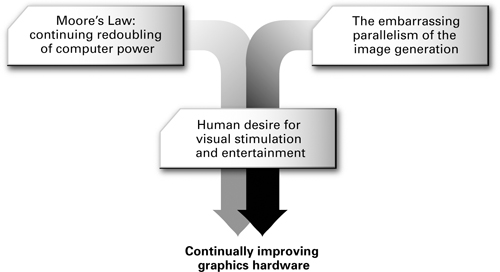
\includegraphics[width=1\linewidth]{Images/fig1_2.jpg}
    \caption{Forces Driving Graphics Hardware Innovation}
    \label{fig:1-2}
\end{figure}

The second force is the vast amount of computation required to simulate the world around us. Our eyes consume and our brains comprehend images of our 3D world at an astounding rate and with startling acuity. We are unlikely ever to reach a point where computer graphics becomes a substitute for reality. Reality is just too real. Undaunted, computer graphics practitioners continue to rise to the challenge. Fortunately, generating images is an embarrassingly parallel problem. What we mean by "embarrassingly parallel" is that graphics hardware designers can repeatedly split up the problem of creating realistic images into more chunks of work that are smaller and easier to tackle. Then hardware engineers can arrange, in parallel, the ever-greater number of transistors available to execute all these various chunks of work.

Our third force is the sustained desire we all have to be stimulated and entertained visually. This is the force that "connects" the source of our continued redoubling of computer hardware resources to the task of approximating visual reality ever more realistically than before.

As Figure \ref{fig:1-2} illustrates, these insights let us confidently predict that computer graphics hardware is going to get much faster. These innovations whet our collective appetite for more interactive and compelling 3D experiences. Satisfying this demand is what motivated the development of the Cg language.

\subsection{Four Generations of Computer Graphics Hardware}

In the mid-1990s, the world's fastest graphics hardware consisted of multiple chips that worked together to render images and display them to a screen. The most complex computer graphics systems consisted of dozens of chips spread over several boards. As time progressed and semiconductor technology improved, hardware engineers incorporated the functionality of complicated multichip designs into a single graphics chip. This development resulted in tremendous economies of integration and scale.

You may be surprised to learn that the GPU now exceeds the CPU in the number of transistors present in each microchip. Transistor count is a rough measure of how much computer hardware is devoted to a microchip. For example, Intel packed its 2.4 GHz Pentium 4 with 55 million transistors; NVIDIA used over 125 million transistors in the original GeForce FX GPU.

NVIDIA introduced the term "GPU" in the late 1990s when the legacy term "VGA controller" was no longer an accurate description of the graphics hardware in a PC. IBM had introduced Video Graphics Array (VGA) hardware in 1987. At that time, the VGA controller was what we now call a "dumb" frame buffer. This meant that the CPU was responsible for updating all the pixels. Today the CPU rarely manipulates pixels directly. Instead, graphics hardware designers build the "smarts" of pixel updates into the GPU.

Industry observers have identified four generations of GPU evolution so far. Each generation delivers better performance and evolving programmability of the GPU feature set. Each generation also influences and incorporates the functionality of the two major 3D programming interfaces, OpenGL and DirectX. OpenGL is an open standard for 3D programming for Windows, Linux, UNIX, and Macintosh computers. DirectX is an evolving set of Microsoft multimedia programming interfaces, including Direct3D for 3D programming.

\subsection*{Pre-GPU Graphics Acceleration}

Prior to the introduction of GPUs, companies such as Silicon Graphics (SGI) and Evans \& Sutherland designed specialized and expensive graphics hardware. The graphics systems developed by these companies introduced many of the concepts, such as vertex transformation and texture mapping, that we take for granted today. These systems were very important to the historical development of computer graphics, but because they were so expensive, they did not achieve the mass-market success of single-chip GPUs designed for PCs and video game consoles. Today, GPUs are far more powerful and much cheaper than any prior systems.

\subsection*{First-Generation GPUs}

The first generation of GPUs (up to 1998) includes NVIDIA's TNT2, ATI's Rage, and 3dfx's Voodoo3. These GPUs are capable of rasterizing pre-transformed triangles and applying one or two textures. They also implement the DirectX 6 feature set. When running most 3D and 2D applications, these GPUs completely relieve the CPU from updating individual pixels. However, GPUs in this generation suffer from two clear limitations. First, they lack the ability to transform vertices of 3D objects; instead, vertex transformations occur in the CPU. Second, they have a quite limited set of math operations for combining textures to compute the color of rasterized pixels.

\subsection*{Second-Generation GPUs}

The second generation of GPUs (1999–2000) includes NVIDIA's GeForce 256 and GeForce2, ATI's Radeon 7500, and S3's Savage3D. These GPUs offload 3D vertex transformation and lighting (T\&L) from the CPU. Fast vertex transformation was one of the key capabilities that differentiated high-end workstations from PCs prior to this generation. Both OpenGL and DirectX 7 support hardware vertex transformation. Although the set of math operations for combining textures and coloring pixels expanded in this generation to include cube map textures and signed math operations, the possibilities are still limited. Put another way, this generation is more configurable, but still not truly programmable.

\subsection*{Third-Generation GPUs}

The third generation of GPUs (2001) includes NVIDIA's GeForce3 and GeForce4 Ti, Microsoft's Xbox, and ATI's Radeon 8500. This generation provides vertex programmability rather than merely offering more configurability. Instead of supporting the conventional transformation and lighting modes specified by OpenGL and DirectX 7, these GPUs let the application specify a sequence of instructions for processing vertices. Considerably more pixel-level configurability is available, but these modes are not powerful enough to be considered truly programmable. Because these GPUs support vertex programmability but lack true pixel programmability, this generation is transitional. DirectX 8 and the multivendor ARB\_vertex\_program OpenGL extension expose vertex-level programmability to applications. DirectX 8 pixel shaders and various vendor-specific OpenGL extensions expose this generation's fragment-level configurability.

\subsection*{Fourth-Generation GPUs}

The fourth and current generation of GPUs (2002 and on) includes NVIDIA's GeForce FX family with the CineFX architecture and ATI's Radeon 9700. These GPUs provide both vertex-level and pixel-level programmability. This level of programmability opens up the possibility of offloading complex vertex transformation and pixel-shading operations from the CPU to the GPU. DirectX 9 and various OpenGL extensions expose the vertex-level and pixel-level programmability of these GPUs. This is the generation of GPUs where Cg gets really interesting. Table \ref{table:1-1} lists selected NVIDIA GPUs representing these various GPU generations.

\FloatBarrier
\begin{table}
\centering
\begin{tabular}{ |c|c|c|c|c|c|c|c| } 
 \hline
 Generation & Year & Product Name & Process & Transistors & Antialiasing Fill Rate & Polygon Rate & Note \\
 \hline
 First & Late 1998 & RIVA TNT & 0.25 m & 7 M & 50 M & 6 M & [1] \\
 First & Early 1999 & RIVA TNT2 & 0.22 m & 9 M & 75 M & 9 M & [2] \\
 Second & Late 1999 & GeForce 256 & 0.22 m & 23 M & 120 M & 15 M & [3] \\
 Second & Early 2000 & GeForce2 & 0.18 m & 25 M & 200 M & 25 M & [4] \\
 Third & Early 2001 & GeForce3 & 0.15 m & 57 M & 800 M & 30 M & [5] \\
 Third & Early 2002 & GeForce4 Ti & 0.15 m & 63 M & 1200 M & 60 M & [6] \\
 Fourth & Early 2003 & GeForce FX & 0.13 m & 125 M & 2000 M & 200 M & [7] \\
 \hline
\end{tabular}
\caption{Features and Performance Evolution of Selected NVIDIA GPUs, by Generation}
\label{table:1-1}

\textbf{Notes}
\begin{itemize}
\item[] 1 Dual texture DirectX 6
\item[] 2 AGP 4×
\item[] 3 Fixed-function vertex hardware, register combiners, cube maps, DirectX 7
\item[] 4 Performance, double data-rate (DDR) memory
\item[] 5 Vertex programs, quad-texturing, texture shaders, DirectX 8
\item[] 6 Performance, antialiasing
\item[] 7 Massive vertex and fragment programmability, floating-point pixels, DirectX 9, AGP 8×
\end{itemize}

\end{table}
\FloatBarrier

The table uses the following terms:

\FloatBarrier
\begin{itemize}
    \item \textbf{Process} —the minimum feature size in microns (m, millionths of a meter) for the semiconductor process used to fabricate each microchip
    \item \textbf{Transistors} —an approximate measure, in millions (M), of the chips' design and manufacturing complexity
    \item \textbf{Antialiasing fill rate} —a GPU's ability to fill pixels, measured in millions (M) of 32-bit RGBA pixels per second, assuming two-sample antialiasing; numbers in italics indicate fill rates that are de-rated because the hardware lacks true antialiased rendering
    \item \textbf{Polygon rate} —a GPU's ability to draw triangles, measured in millions (M) of triangles per second
\end{itemize}
\FloatBarrier

The notes highlight the most significant improvements in each design. Performance rates may not be comparable with designs from other hardware vendors.

Future GPUs will further generalize the programmable aspects of current GPUs, and Cg will make this additional programmability easy to use.

\begin{figure}
    \centering
    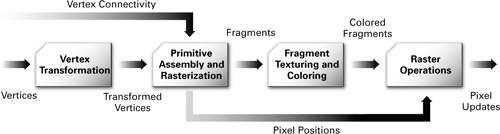
\includegraphics[width=1\linewidth]{Images/fig1_3.jpg}
    \caption{The Graphics Hardware Pipeline}
    \label{fig:1-3}
\end{figure}

\subsection{The Graphics Hardware Pipeline}

A pipeline is a sequence of stages operating in parallel and in a fixed order. Each stage receives its input from the prior stage and sends its output to the subsequent stage. Like an assembly line where dozens of automobiles are manufactured at the same time, with each automobile at a different stage of the line, a conventional graphics hardware pipeline processes a multitude of vertices, geometric primitives, and fragments in a pipelined fashion.

Figure \ref{fig:1-3} shows the graphics hardware pipeline used by today's GPUs. The 3D application sends the GPU a sequence of vertices batched into geometric primitives: typically polygons, lines, and points. As shown in Figure \ref{fig:1-4}, there are many ways to specify geometric primitives.

Every vertex has a position but also usually has several other attributes such as a color, a secondary (or specular) color, one or multiple texture coordinate sets, and a normal vector. The normal vector indicates what direction the surface faces at the vertex, and is typically used in lighting calculations.

\subsection*{Vertex Transformation}

Vertex transformation is the first processing stage in the graphics hardware pipeline. Vertex transformation performs a sequence of math operations on each vertex. These operations include transforming the vertex position into a screen position for use by the rasterizer, generating texture coordinates for texturing, and lighting the vertex to determine its color. We will explain many of these tasks in subsequent chapters.

\begin{figure}
    \centering
    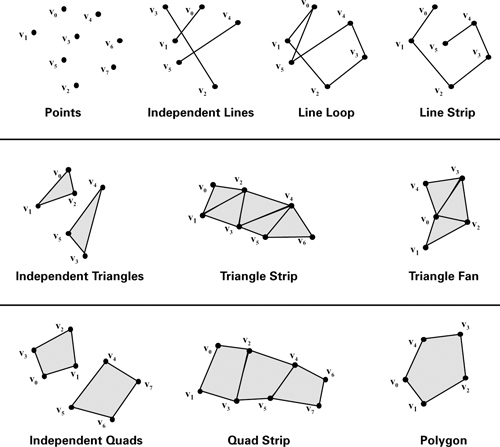
\includegraphics[width=1\linewidth]{Images/fig1_4.jpg}
    \caption{Types of Geometric Primitives}
    \label{fig:1-4}
\end{figure}

\subsection*{Primitive Assembly and Rasterization}

The transformed vertices flow in sequence to the next stage, called primitive assembly and rasterization. First, the primitive assembly step assembles vertices into geometric primitives based on the geometric primitive batching information that accompanies the sequence of vertices. This results in a sequence of triangles, lines, or points. These primitives may require clipping to the view frustum (the view's visible region of 3D space), as well as any enabled application-specified clip planes. The rasterizer may also discard polygons based on whether they face forward or backward. This process is known as culling.

Polygons that survive these clipping and culling steps must be rasterized. Rasterization is the process of determining the set of pixels covered by a geometric primitive. Polygons, lines, and points are each rasterized according to the rules specified for each type of primitive. The results of rasterization are a set of pixel locations as well as a set of fragments. There is no relationship between the number of vertices a primitive has and the number of fragments that are generated when it is rasterized. For example, a triangle made up of just three vertices could take up the entire screen, and therefore generate millions of fragments!

Earlier, we told you to think of a fragment as a pixel if you did not know precisely what a fragment was. At this point, however, the distinction between a fragment and a pixel becomes important. The term pixel is short for "picture element." A pixel represents the contents of the frame buffer at a specific location, such as the color, depth, and any other values associated with that location. A fragment is the state required potentially to update a particular pixel.

The term "fragment" is used because rasterization breaks up each geometric primitive, such as a triangle, into pixel-sized fragments for each pixel that the primitive covers. A fragment has an associated pixel location, a depth value, and a set of interpolated parameters such as a color, a secondary (specular) color, and one or more texture coordinate sets. These various interpolated parameters are derived from the transformed vertices that make up the particular geometric primitive used to generate the fragments. You can think of a fragment as a "potential pixel." If a fragment passes the various rasterization tests (in the raster operations stage, which is described shortly), the fragment updates a pixel in the frame buffer.

\subsection*{Interpolation, Texturing, and Coloring}

Once a primitive is rasterized into a collection of zero or more fragments, the interpolation, texturing, and coloring stage interpolates the fragment parameters as necessary, performs a sequence of texturing and math operations, and determines a final color for each fragment. In addition to determining the fragment's final color, this stage may also determine a new depth or may even discard the fragment to avoid updating the frame buffer's corresponding pixel. Allowing for the possibility that the stage may discard a fragment, this stage emits one or zero colored fragments for every input fragment it receives.

\subsection*{Raster Operations}

The raster operations stage performs a final sequence of per-fragment operations immediately before updating the frame buffer. These operations are a standard part of OpenGL and Direct3D. During this stage, hidden surfaces are eliminated through a process known as depth testing. Other effects, such as blending and stencil-based shadowing, also occur during this stage.

\begin{figure}
    \centering
    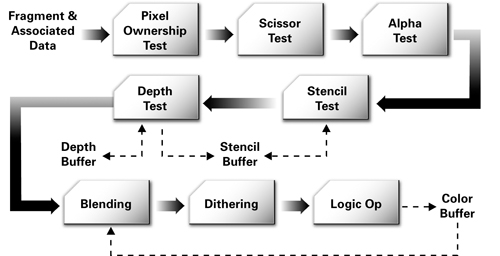
\includegraphics[width=1\linewidth]{Images/fig1_5.jpg}
    \caption{Standard OpenGL and Direct3D Raster Operations}
    \label{fig:1-5}
\end{figure}

The raster operations stage checks each fragment based on a number of tests, including the scissor, alpha, stencil, and depth tests. These tests involve the fragment's final color or depth, the pixel location, and per-pixel values such as the depth value and stencil value of the pixel. If any test fails, this stage discards the fragment without updating the pixel's color value (though a stencil write operation may occur). Passing the depth test may replace the pixel's depth value with the fragment's depth. After the tests, a blending operation combines the final color of the fragment with the corresponding pixel's color value. Finally, a frame buffer write operation replaces the pixel's color with the blended color. Figure \ref{fig:1-5} shows this sequence of operations.

Figure \ref{fig:1-5} shows that the raster operations stage is actually itself a series of pipeline stages. In fact, all of the previously described stages can be broken down into substages as well.

\subsection*{Visualizing the Graphics Pipeline}

Figure \ref{fig:1-6} depicts the stages of the graphics pipeline. In the figure, two triangles are rasterized. The process starts with the transformation and coloring of vertices. Next, the primitive assembly step creates triangles from the vertices, as the dotted lines indicate. After this, the rasterizer "fills in" the triangles with fragments. Finally, the register values from the vertices are interpolated and used for texturing and coloring. Notice that many fragments are generated from just a few vertices.

\begin{figure}
    \centering
    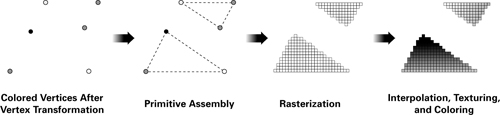
\includegraphics[width=1\linewidth]{Images/fig1_6.jpg}
    \caption{Visualizing the Graphics Pipeline}
    \label{fig:1-6}
\end{figure}

\subsection{The Programmable Graphics Pipeline}

The dominant trend in graphics hardware design today is the effort to expose more programmability within the GPU. Figure \ref{fig:1-7} shows the vertex processing and fragment processing stages in the pipeline of a programmable GPU.

\begin{figure}
    \centering
    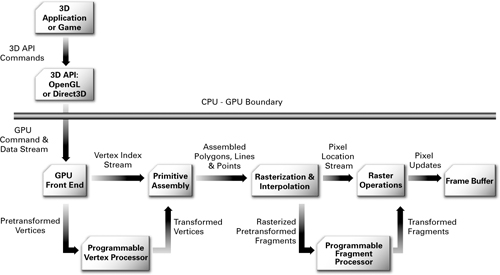
\includegraphics[width=1\linewidth]{Images/fig1_7.jpg}
    \caption{The Programmable Graphics Pipeline}
    \label{fig:1-7}
\end{figure}

Figure \ref{fig:1-7} shows more detail than Figure \ref{fig:1-3}, but more important, it shows the vertex and fragment processing broken out into programmable units. The programmable vertex processor is the hardware unit that runs your Cg vertex programs, whereas the programmable fragment processor is the unit that runs your Cg fragment programs.

As explained in Section 1.2.2, GPU designs have evolved, and the vertex and fragment processors within the GPU have transitioned from being configurable to being programmable. The descriptions in the next two sections present the critical functional features of programmable vertex and fragment processors.

\subsection*{The Programmable Vertex Processor}

Figure \ref{fig:1-8} shows a flow chart for a typical programmable vertex processor. The data-flow model for vertex processing begins by loading each vertex's attributes (such as position, color, texture coordinates, and so on) into the vertex processor. The vertex processor then repeatedly fetches the next instruction and executes it until the vertex program terminates. Instructions access several distinct sets of registers banks that contain vector values, such as position, normal, or color. The vertex attribute registers are read-only and contain the application-specified set of attributes for the vertex. The temporary registers can be read and written and are used for computing intermediate results. The output result registers are write-only. The program is responsible for writing its results to these registers. When the vertex program terminates, the output result registers contain the newly transformed vertex. After triangle setup and rasterization, the interpolated values for each register are passed to the fragment processor.

\begin{figure}
    \centering
    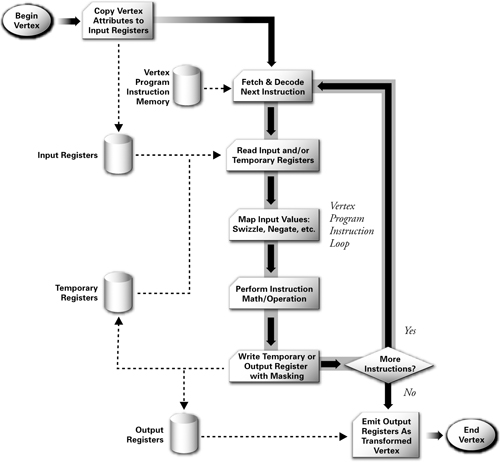
\includegraphics[width=1\linewidth]{Images/fig1_8.jpg}
    \caption{Programmable Vertex Processor Flow Chart}
    \label{fig:1-8}
\end{figure}

Most vertex processing uses a limited palette of operations. Vector math operations on floating-point vectors of two, three, or four components are necessary. These operations include add, multiply, multiply-add, dot product, minimum, and maximum. Hardware support for vector negation and component-wise swizzling (the ability to reorder vector components arbitrarily) generalizes these vector math instructions to provide negation, subtraction, and cross products. Component-wise write masking controls the output of all instructions. Combining reciprocal and reciprocal square root operations with vector multiplication and dot products, respectively, enables vector-by-scalar division and vector normalization. Exponential, logarithmic, and trigonometric approximations facilitate lighting, fog, and geometric computations. Specialized instructions can make lighting and attenuation functions easier to compute.

Further functionality, such as relative addressing of constants and flow-control support for branching and looping, is also available in more recent programmable vertex processors.

\subsection*{The Programmable Fragment Processor}

Programmable fragment processors require many of the same math operations as programmable vertex processors do, but they also support texturing operations. Texturing operations enable the processor to access a texture image using a set of texture coordinates and then to return a filtered sample of the texture image.

Newer GPUs offer full support for floating-point values; older GPUs have more limited fixed-point data types. Even when floating-point operations are available, fragment operations are often more efficient when using lower-precision data types. GPUs must process so many fragments at once that arbitrary branching is not available in current GPU generations, but this is likely to change over time as hardware evolves. Cg still allows you to write fragment programs that branch and iterate by simulating such constructs with conditional assignment operations or loop unrolling.

Figure \ref{fig:1-9} shows the flow chart for a current programmable fragment processor. As with a programmable vertex processor, the data flow involves executing a sequence of instructions until the program terminates. Again, there is a set of input registers. However, rather than vertex attributes, the fragment processor's read-only input registers contain interpolated per-fragment parameters derived from the per-vertex parameters of the fragment's primitive. Read/write temporary registers store intermediate values. Write operations to write-only output registers become the color and optionally the new depth of the fragment. Fragment program instructions include texture fetches.

\begin{figure}
    \centering
    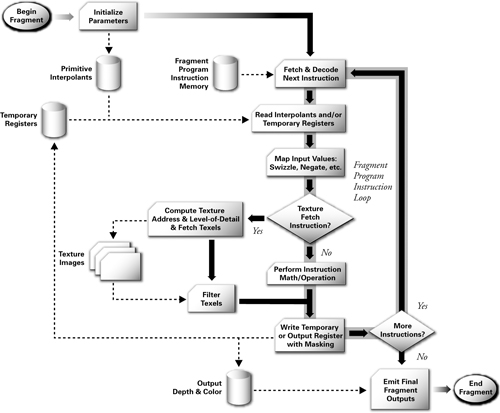
\includegraphics[width=1\linewidth]{Images/fig1_9.jpg}
    \caption{Programmable Fragment Processor Flow Chart}
    \label{fig:1-9}
\end{figure}

\subsection{Cg Provides Vertex and Fragment Programmability}

These two programmable processors in your GPU require you, the application programmer, to supply a program for each processor to execute. What Cg provides is a language and a compiler that can translate your shading algorithm into a form that your GPU's hardware can execute. With Cg, rather than program at the level shown in Figures \ref{fig:1-8} and \ref{fig:1-9}, you can program in a high-level language very similar to C.

\section{Cg's Historical Development}

Cg's heritage comes from three sources, as shown in Figure \ref{fig:1-10}. First, Cg bases its syntax and semantics on the general-purpose C programming language. Second, Cg incorporates many concepts from offline shading languages such as the RenderMan Shading Language, as well as prior hardware shading languages developed by academia. Third, Cg bases its graphics functionality on the OpenGL and Direct3D programming interfaces for real-time 3D.

\begin{figure}
    \centering
    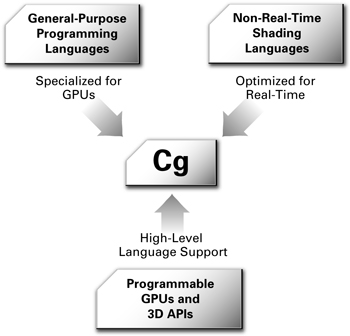
\includegraphics[width=1\linewidth]{Images/fig1_10.jpg}
    \caption{Sources of Cg's Technology Heritage}
    \label{fig:1-10}
\end{figure}

Figure \ref{fig:1-11} shows the general-purpose programming languages, 3D application programming interfaces, and shading languages that inspired Cg's development.

\begin{figure}
    \centering
    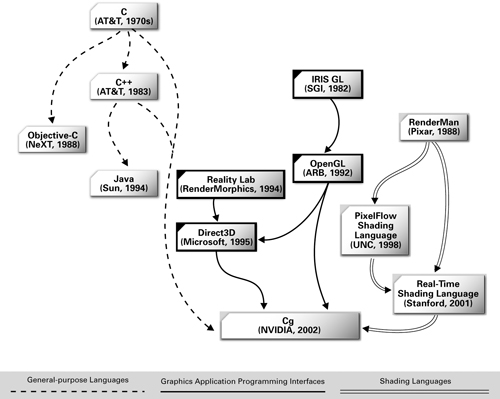
\includegraphics[width=1\linewidth]{Images/fig1_11.jpg}
    \caption{Inspirations for Cg's Development}
    \label{fig:1-11}
\end{figure}

Earlier, we mentioned how Cg leverages C's syntax and semantics. Over the course of this book, you will find that Cg mostly does what C programmers expect. Cg differs from C in situations where either Cg's specialization for GPUs or performance justifies a change.

\subsection{Microsoft and NVIDIA's Collaboration to Develop Cg and HLSL}

NVIDIA and Microsoft collaborated to develop the Cg language. Microsoft calls its implementation High-Level Shading Language, or HLSL for short. HLSL and Cg are the same language but reflect the different names each company uses to identify the language and its underlying technology. HLSL is a part of Microsoft's DirectX Graphics, a component of the DirectX 9 multimedia framework. Direct3D is the 3D component of Microsoft's DirectX Graphics. Cg is independent of the 3D programming interface and fully integrates with either Direct3D or OpenGL. A properly written Cg application can be written once and then work with either OpenGL or Direct3D.

This flexibility means that NVIDIA's Cg implementation provides a way to author programs that work with both dominant 3D programming interfaces and whatever operating system you choose. Cg works whether you choose Windows, Linux, Mac OS X, a game console, or embedded 3D hardware as your 3D computing platform. Cg programs work with hardware from multiple hardware vendors because Cg layers cleanly upon either Direct3D or OpenGL. Cg programs work on programmable GPUs from all the major graphics hardware vendors, such as 3Dlabs, ATI, Matrox, and NVIDIA.

The multivendor, cross-API, and multiplatform nature of the Cg language makes it the best choice when writing programs for programmable GPUs.

\subsection{Noninteractive Shading Languages}

The RenderMan Interface Standard describes the best-known shading language for noninteractive shading. Pixar developed the language in the late 1980s to generate high-quality computer animation with sophisticated shading for films and commercials. Pixar has created a complete rendering system with its implementation of the RenderMan Interface Standard, the offline renderer PRMan (PhotoRealistic RenderMan). The RenderMan Shading Language is just one component of this system.

\subsection*{Shade Trees}

The inspiration for the RenderMan Shading Language came from an earlier idea called shade trees. Rob Cook, then at Lucasfilm Ltd., which later spun off Pixar, published a SIGGRAPH paper about shade trees in 1984. A shade tree organizes various shading operations as nodes within a tree structure. Figure \ref{fig:1-12} shows a shade tree for rendering a copper surface. The leaf nodes are data inputs to the shade tree. The nonleaf nodes represent simple shading operations. During the process of rendering, the renderer evaluates the shade tree associated with a given surface to determine the color of the surface in the rendered image. To evaluate a shade tree, a renderer performs the shading operation associated with the topmost node in the shade tree. However, to evaluate a given node, the renderer must first evaluate the node's child nodes. This rule is applied recursively to evaluate the shade tree fully. The result of a shade tree evaluation at a given point on a surface is the color of that point.

\begin{figure}
    \centering
    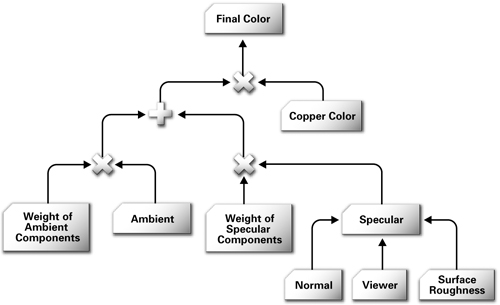
\includegraphics[width=1\linewidth]{Images/fig1_12.jpg}
    \caption{A Shade Tree Example, Based on Rob Cook's Original SIGGRAPH Paper}
    \label{fig:1-12}
\end{figure}

Shade trees grew out of the realization that a single predefined shading model would never be sufficient for all the objects and scenes one might want to render.

Shade tree diagrams are great for visualizing a data flow of shading operations. However, if the shade trees are complex, their diagrams become unwieldy. Researchers at Pixar and elsewhere recognized that each shade tree is a limited kind of program. This realization provided the impetus for a new kind of programming language known as a shading language.

\subsection*{The RenderMan Shading Language}

The RenderMan Shading Language grew out of shade trees and the realization that open-ended control of the appearance of rendered surfaces in the pursuit of photorealism requires programmability.

Today most offline renderers used in actual production have some type of support for a shading language. The RenderMan Shading Language is the most established and best known for offline rendering, and it was significantly overhauled and extended in the late 1990s.

\subsection*{Hardware-Amenable Shading Languages}

A hardware implementation of an algorithm is most efficient when the task decomposes into a long sequence of stages in which each stage's communication is limited to its prior stage and its subsequent stage (that is, when it can be pipelined).

The vertex-based and fragment-based pipeline described in Section 1.2 is extremely amenable to hardware implementation. However, the Reyes algorithm used by PhotoRealistic RenderMan is not very suitable for efficient hardware implementation, primarily due to its higher-level geometry handling. Contemporary GPUs rely completely on a graphics pipeline based on vertices and fragments.

Researchers at the University of North Carolina (UNC) began investigating programmable graphics hardware in the mid-1990s, when UNC was developing a new programmable graphics hardware architecture called PixelFlow. This project fostered a new line of computer graphics research into hardware-amenable shading languages by Marc Olano and others at UNC. Unfortunately, PixelFlow was too expensive and failed commercially.

Subsequently, researchers at Silicon Graphics worked on a system to translate shaders into multiple passes of OpenGL rendering. Although the targeted OpenGL hardware was not programmable in the way GPUs are today, the OpenGL Shader system orchestrates numerous rendering passes to achieve a shader's intended effect.

Researchers at Stanford University, including Kekoa Proudfoot, Bill Mark, Svetoslav Tzvetkov, and Pat Hanrahan, began building a shading language designed specifically for second-generation and third-generation GPUs. This language, known as the Stanford Real-Time Shading Language (RTSL), could compile shaders written in RTSL into one or more OpenGL rendering passes.

The research at Stanford inspired NVIDIA's own effort to develop a commercial-quality hardware-amenable shading language. Bill Mark joined NVIDIA in 2001 to lead the effort to define and implement the shading language we now call Cg. During this time, NVIDIA collaborated with Microsoft to agree on a common language syntax and feature set.

\subsection{Programming Interfaces for 3D Graphics}

The third influence on Cg was the pair of standard 3D programming interfaces, OpenGL and Direct3D. The influence of these programming interfaces on Cg is ongoing, as is explained in the next section.

\section{The Cg Environment}

Cg is just one component of the overall software and hardware infrastructure for rendering complex 3D scenes with programmable GPUs at real-time rates. This section explains how Cg interacts with actual 3D applications and games.

\subsection{Standard 3D Programming Interfaces: OpenGL and Direct3D}

In the old days of 3D graphics on a PC (before there were GPUs), the CPU handled all the vertex transformation and pixel-pushing tasks required to render a 3D scene. The graphics hardware provided only the buffer of pixels that the hardware displayed to the screen. Programmers had to implement their own 3D graphics rendering algorithms in software. In a sense, everything about vertex and fragment processing back then was completely programmable. Unfortunately, the CPU was too slow to produce compelling 3D effects.

These days, 3D applications no longer implement their own 3D rendering algorithms using the CPU; rather, they rely on either OpenGL or Direct3D, the two standard 3D programming interfaces, to communicate rendering commands to the GPU.

\subsection*{OpenGL}
In the early 1990s, Silicon Graphics developed OpenGL in coordination with an organization called the OpenGL Architecture Review Board (ARB), which comprised all the major computer graphics system vendors. Originally, OpenGL ran only on powerful UNIX graphics workstations. Microsoft, a founding member of the ARB, then implemented OpenGL as a way to support 3D graphics for its Windows NT operating system. Microsoft later added OpenGL support to Windows 95 and all of Microsoft's desktop operating systems.

OpenGL is not limited to a single operating or windowing system. In addition to supporting UNIX workstations and Windows PCs, OpenGL is supported by Apple for its Macintosh personal computers. Linux users can use either the Mesa open-source implementation of OpenGL or a hardware-accelerated implementation such as NVIDIA's OpenGL driver for Linux. This flexibility makes OpenGL the industry's best cross-platform programming interface for 3D graphics.

Over the last decade, OpenGL has evolved along with graphics hardware. OpenGL is extensible, meaning that OpenGL implementers can add new functionality to OpenGL in an incremental way. Today, scores of OpenGL extensions provide access to all the latest GPU features. This includes ARB-standardized extensions for vertex and fragment programmability. As extensions are established, they are often rolled into the core OpenGL standard so that the standard as a whole advances. At the time of this writing, the current version of OpenGL is 1.4. Ongoing work to evolve OpenGL is underway in various OpenGL ARB working groups. This work includes both assembly-level and high-level programmable interfaces. Because Cg operates as a layer above such interfaces, it will continue to function with future revisions of OpenGL in a compatible manner.

\subsection*{Direct3D}

Microsoft began developing the Direct3D programming interface about 1995 as part of its DirectX multimedia initiative. Direct3D is one of the programming interfaces that make up DirectX. Microsoft introduced DirectX and Direct3D to jump-start the consumer market for 3D graphics, particularly gaming, on Windows PCs. Microsoft's Xbox game console also supports Direct3D. Direct3D is the most popular graphics API for games on Windows, due to its history of closely matching the capabilities of available graphics hardware.

Every year or so, Microsoft has updated DirectX, including Direct3D, to keep up with the rapid pace of PC hardware innovation. The current version of DirectX at the time of this writing is DirectX 9, which includes HLSL, Microsoft's implementation of the same language syntax and constructs found in Cg.

\subsection*{3D Programming Interface Détente}

A few years ago, OpenGL and Direct3D competed to see which programming interface would dominate, particularly in the domain of Windows PCs. The competition continues to be good for both programming interfaces, and each has improved in performance, quality, and functionality. In the area of GPU programmability that Cg addresses, both programming interfaces have comparable capabilities. This is because both OpenGL and Direct3D run on the same GPU hardware and the graphics hardware determines the available functionality and performance. OpenGL has a slight advantage in functionality because hardware vendors are better able to expose their entire feature set through OpenGL, though vendor-specific extensions do add some complexity for developers.

Most software developers now choose a 3D programming interface based on programmer preference, history, and their target market and hardware platform, rather than on technical grounds.

Cg supports either programming interface. You can write Cg programs so that they work with either the OpenGL or Direct3D programming interface. This is a huge boon for 3D content developers. They can pair their 3D content with programs written in Cg and then render the content no matter what programming interface the final application uses for 3D rendering.

\subsection{The Cg Compiler and Runtime}

No GPU can execute Cg programs directly from their textual form. A process known as compilation must translate Cg programs into a form that the GPU can execute. The Cg compiler first translates your Cg program into a form accepted by the application's choice of 3D programming interface, either OpenGL or Direct3D. Then your application transfers the OpenGL or Direct3D translation of your Cg program to the GPU using the appropriate OpenGL or Direct3D commands. The OpenGL or Direct3D driver performs the final translation into the hardware-executable form your GPU requires.

The details of this translation depend on the combined capabilities of the GPU and 3D programming interface. How a Cg program compiles its intermediate OpenGL or Direct3D form depends on the type and generation of GPU in your computer. It may be that your GPU is not capable of supporting a particular valid Cg program because of limitations of the GPU itself. For example, your Cg fragment program will not compile if your program accesses more texture units than your target GPU supports.

\subsection*{Support for Dynamic Compilation}

When you compile a program with a conventional programming language such as C or C++, compilation is an offline process. Your compiler compiles the program into an executable that runs directly on the CPU. Once compiled, your program does not need to be recompiled, unless you change the program code. We call this static compilation.

Cg is different because it encourages dynamic compilation, although static compilation is also supported. The Cg compiler is not a separate program but part of a library known as the Cg runtime. 3D applications and games using Cg programs must link with the Cg runtime. Applications using Cg then call Cg runtime routines, all prefixed with the letters cg , to compile and manipulate Cg programs. Dynamic compilation allows Cg programs to be optimized for the particular model of GPU installed in the user's machine.

\subsection*{CgGL and CgD3D, the 3D-API-Specific Cg Libraries}

In addition to the core Cg runtime, Cg provides two closely related libraries. If your application uses OpenGL, you will use the CgGL library to invoke the appropriate OpenGL routines to pass your translated Cg program to the OpenGL driver. Likewise, if your application uses Direct3D, you will use the CgD3D library to invoke the appropriate Direct3D routines to pass your translated Cg program to the Direct3D driver. Normally, you would use either the CgGL or the CgD3D library, but not both, because most applications use either OpenGL or Direct3D, not both.

Compared with the core Cg runtime library that contains the Cg compiler, the CgGL and CgD3D libraries are relatively small. Their job is to make the appropriate OpenGL or Direct3D calls for you to configure Cg programs for execution. These calls transfer a translated Cg program to the appropriate driver that will further translate the program into a form your GPU can execute. For the most part, the CgGL and CgD3D libraries have similar routines. The routines in the CgGL library begin with cgGL ; the routines in the CgD3D library begin with cgD3D .

\subsection*{How the Cg Runtime Fits into Your Application}

Figure \ref{fig:1-13} shows how a typical 3D application uses the Cg libraries. If you are a programmer, you will want to learn more about the Cg runtime and the specific library for the 3D API your application uses to render 3D graphics. Most of this book focuses on the Cg language itself and on how to write Cg programs, but Appendix B has more information about the Cg runtime library.

\begin{figure}
    \centering
    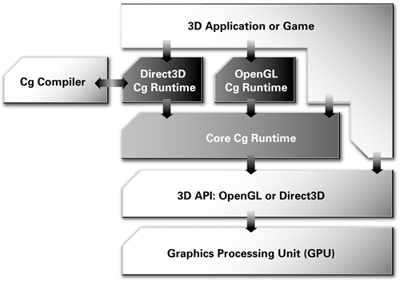
\includegraphics[width=1\linewidth]{Images/fig1_13.jpg}
    \caption{How Cg Fits into a Standard Cg Application}
    \label{fig:1-13}
\end{figure}

\subsection{The CgFX Toolkit and File Format}

Cg programs need 3D models, textures, and other data to operate on. A Cg program without any associated data is useless. Cg programs and data also require the correct 3D programming interface configuration and state. It is often helpful to have a way to bundle all the information required to render a 3D model, including its associated Cg program.

\subsection*{What CgFX Provides}

CgFX is a standardized file format for representing complete effects and appearances. As they did with Cg, Microsoft and NVIDIA collaborated to develop the CgFX format. CgFX files are text-based, with a syntax that is a superset of Cg's, and may contain any number of Cg programs. The .fx suffix identifies CgFX files. A CgFX file describes the complete render state for a particular effect: multiple passes, texture states, and any number of individual vertex and fragment programs may be defined to create a complete appearance or effect. An accompanying development toolkit is provided for using and parsing CgFX files. The toolkit exposes user-interface hooks to host applications, so that CgFX-aware applications can automatically supply meaningful controls and semantics to users and developers alike.

Cg programs describe the vertex or fragment processing that takes place in a single rendering pass, but some complex shading algorithms require multiple rendering passes. CgFX offers a format to encode complex multipass effects, including designating which Cg program is used for each rendering pass.

More specifically, CgFX supports three additional capabilities beyond what the core Cg language supports:

\FloatBarrier
\begin{enumerate}
\item CgFX provides a mechanism for specifying multiple rendering passes and optional multiple implementations for a single effect.
\item CgFX allows you to specify nonprogrammable rendering states, such as alpha-test modes and texture-filtering. The settings for these render states may take the form of simple expressions, which are evaluated on the CPU when the effect is initialized.
\item CgFX allows annotations to be added to shaders and shader parameters. These annotations provide additional information to applications, including content creation applications. For example, an annotation can specify the allowed range of values for a shader parameter.
\end{enumerate}
\FloatBarrier

\subsection*{Multiple Shader Instancing}

The CgFX file format encapsulates multiple implementations of Cg programs for a given shader. This means you can have one Cg shader program written for a third-generation or fourth-generation GPU, while also including a simpler program that supports a less capable, second-generation GPU. An application loading the CgFX file can determine at runtime the most appropriate shader implementation to use based on the computer's available GPU.

Multiple instancing of Cg programs with CgFX is one way to address the functional variations in GPUs of different generations or different hardware vendors. Multiple instancing also lets you develop a Cg program specialized for a particular 3D API—for example, if OpenGL exposes extra functionality through an extension. Cg programs specialized for Direct3D, standard OpenGL, or OpenGL with extensions can all be contained in a single CgFX file.

\subsection*{CgFX and Digital Content Creation}

The CgFX Toolkit consists of the CgFX compiler, which supports the full CgFX syntax; the CgFX runtime API, for loading and manipulating CgFX files; and plug-in modules for major digital content creation (DCC) applications such as Alias|Wavefront's Maya and Discreet's 3ds max. Figure \ref{fig:1-14} shows these applications making use of CgFX. Softimage|XSI 3.0 provides direct support for Cg compilation in its Render Tree.

\begin{figure}
    \centering
    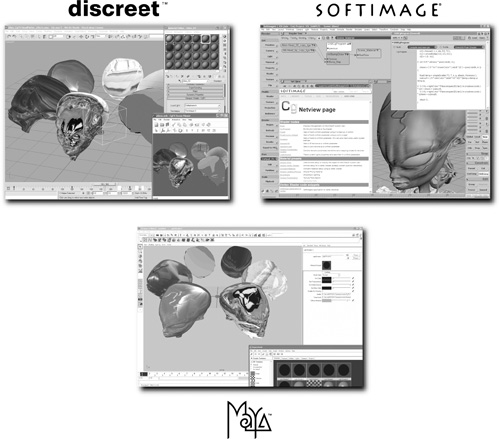
\includegraphics[width=1\linewidth]{Images/fig1_14.jpg}
    \caption{Digital Content Creation Applications That Use Cg and CgFX}
    \label{fig:1-14}
\end{figure}

Prior to CgFX, there was no standard way for a DCC application to export 3D content with all the associated shading knowledge necessary to render the content in real time. Now the major DCC applications use CgFX in their content creation process and support the CgFX file format. This means that CgFX can significantly improve the artistic workflow from DCC applications to real-time games and other 3D applications. Using CgFX, artists can view and tweak Cg shaders and associated 3D content to see, from within the DCC tool of their choice, how their work will appear in a 3D game or application.

\subsection*{How CgFX Fits into Your Application}

Figure \ref{fig:1-15} shows how a CgFX file containing multiple instanced shaders is used by an application in conjunction with the Cg runtime and your choice of rendering API. Most of this book focuses on the Cg language itself and on how to write Cg programs, rather than CgFX, but see Appendix C for more information about the CgFX file format and its associated runtime API.

\begin{figure}
    \centering
    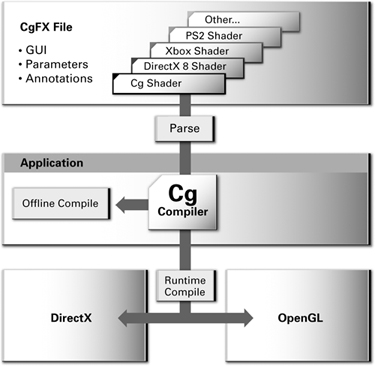
\includegraphics[width=1\linewidth]{Images/fig1_15.jpg}
    \caption{How CgFX Fits into a Standard Application}
    \label{fig:1-15}
\end{figure}

\subsection*{Onward to the Tutorial}

Having finished this introduction to the Cg programming language, you are now ready to take on the tutorial chapters, which will teach you how to write Cg programs.

\section{Exercises}

The exercises at the end of each chapter help you review your knowledge and develop practical programming skills.

\FloatBarrier
\begin{enumerate}
    \item \textbf{Answer this:} Name two standard 3D programming interfaces for which you can compile Cg programs. What operating systems does each programming interface support?
    \item \textbf{Answer this:} What are the major stages of the graphics pipeline? In what order are the stages arranged?
    \item \textbf{Answer this:} Where do vertex and fragment programs fit into the pipeline?
    \item \textbf{Answer this:} What is a vertex? What is a fragment? Distinguish a fragment from a pixel.
    \item \textbf{Try this yourself:} We haven't begun writing Cg programs yet (we'll get there soon enough in the next chapter), so take a break and watch a good feature-length computer graphics animation such as Monsters, Inc.
\end{enumerate}
\FloatBarrier

\section{Further Reading}

Cg builds on a host of concepts in computer language design, computer hardware design, and computer graphics. Doing justice to all these contributions in the context of this tutorial is not always practical. What we attempt in the "Further Reading" section at the end of each chapter is to offer you pointers to learn more about the contributions that underlie the topics in each chapter.
\par
There are plenty of books on C. \textit{The C Programming Language, Third Edition} (Prentice Hall, 2000), by Brian Kernighan and Dennis Ritchie, is a classic; the authors invented the C language. Cg includes concepts from both C and C++. There now may actually be more books about C++ than about C. The classic C++ book is \textit{The C++ Programming Language, Third Edition} (Addison-Wesley, 2000), by Bjarne Stroustrup, who invented the language.

To learn more about the RenderMan Shading Language, read \textit{The RenderMan Companion: A Programmer's Guide to Realistic Computer Graphics} (Addison-Wesley, 1989), by Steve Upstill. Pat Hanrahan and Jim Lawson published a SIGGRAPH paper about RenderMan called "A Language for Shading and Lighting Calculations" (ACM Press) in 1990.

Robert Cook's 1984 SIGGRAPH paper titled "Shade Trees" (ACM Press) motivated the development of RenderMan.

The development of programmable graphics hardware and its associated languages has been an active and fruitful research area for almost a decade. Anselmo Lastra, Steven Molnar, Marc Olano, and Yulan Wang at UNC published an early research paper in 1995 titled "Real-Time Programmable Shading" (ACM Press). Researchers at UNC also published several papers about their programmable PixelFlow graphics architecture. Marc Olano and Anselmo Lastra published a SIGGRAPH paper titled "A Shading Language on Graphics Hardware: The PixelFlow Shading System" (ACM Press) in 1998.

Kekoa Proudfoot, Bill Mark, Svetoslav Tzvetkov, and Pat Hanrahan published a SIGGRAPH paper in 2001 titled "A Real-Time Procedural Shading System for Programmable Graphics Hardware" (ACM Press) that describes a GPU-oriented shading language developed at Stanford.

\textit{Real-Time Rendering, Second Edition} (A. K. Peters, 2002), written by Eric Haines and Tomas Akenine-Möller, is an excellent resource for further information about graphics hardware and interactive techniques.

\textit{The OpenGL Graphics System: A Specification} documents the OpenGL 3D programming interface. The best tutorial for learning OpenGL programming is the \textit{OpenGL Programming Guide: The Official Guide to Learning OpenGL, Third Edition} (Addison-Wesley, 1999), by Mason Woo, Jackie Neider, Tom Davis, and Dave Shreiner. The \textbf{www.opengl.org} Web site serves up much more information about OpenGL.

Documentation for the Direct3D programming interface is available from Microsoft's \textbf{msdn.microsoft.com} Web site.

NVIDIA provides further information about the Cg runtime, CgFX, and Cg itself on its Developer Web site at \textbf{developer.nvidia.com/Cg}.

\chapter{The Simplest Programs}

This chapter introduces Cg programming through a series of simple vertex and fragment programs. The chapter has the following four sections:

\FloatBarrier
\begin{itemize}
    \item \textbf{"A Simple Vertex Program"} presents a straightforward vertex program and explains the basic elements and syntax of the Cg language.
    \item \textbf{"Compiling Your Example"} explains how to compile programs for different GPUs, using the concept of profiles.
    \item \textbf{"A Simple Fragment Program"} defines a basic fragment program and introduces fragment profiles.
    \item \textbf{"Rendering with Your Vertex and Fragment Program Examples"} shows how to render simple geometry with OpenGL or Direct3D. This section also mentions the concept of clipping.
\end{itemize}
\FloatBarrier

\section{A Simple Vertex Program}

Green is the color associated with inexperience and growth, so a Cg program for rendering a green 2D triangle is a fitting way to start learning Cg.

Example 2-1 shows the complete source code for your first vertex program in Cg. Source code examples in this book use \textbf{boldface} to indicate Cg keywords, built-in functions, and built-in data types. This notation will help you identify words in programs that have special meaning to the Cg compiler. In addition, comments in code samples are set in gray type, to distinguish them from the rest of the code. Comments in Cg work just as in C++: you can use the \textbf{/*} and \textbf{*/} delimiters, or you can precede comments with the \textbf{//} characters.

\subsection*{The Naming Convention for Examples}

The vertex program in Example 2-1 is quite simple. The "\textbf{C2E1v}" prefix used in various parts of the program stands for "Chapter 2, Example 1 vertex program." We use this notation to make it easier to find examples across chapters and in the accompanying software framework. This convention makes it easier to keep track of the various examples in this book, but it is not a requirement of the Cg language itself and indeed is not a convention intended for your own programs.

\FloatBarrier
\begin{lstlisting}[caption=Example 2-1. The \textbf{C2E1v\_green} Vertex Program]
struct C2E1v_Output {
  float4 position : POSITION;
  float4 color    : COLOR;
};

C2E1v_Output C2E1v_green(float2 position : POSITION)
{
  C2E1v_Output OUT;
  OUT.position = float4(position, 0, 1);
  OUT.color    = float4(0, 1, 0, 1);  // RGBA green
  return OUT;
}
\end{lstlisting}
\FloatBarrier

If you are familiar with C or C++, you can probably deduce what the program does. The program assigns the vertex's incoming 2D position to the vertex's output 2D position. In addition, it assigns the RGBA (red, green, blue, alpha) constant representing green to the output color of the vertex.

\subsection{Output Structures}

The \textbf{C2E1v\_green} program begins with this declaration:

\FloatBarrier
\begin{lstlisting}
struct C2E1v_Output {
  float4 position : POSITION;
  float4 color : COLOR;
};
\end{lstlisting}
\FloatBarrier

This declaration is for a special structure known as an output structure. This structure contains the bundle of values that represent the output (or result) of a given Cg program.

A program written in a general-purpose CPU language such as C can perform a wide variety of tasks, such as reading and writing files, soliciting input from users, printing text, displaying graphics, and communicating over a network. Cg programs, on the other hand, are limited to outputting a bundle of values. A Cg program's output structure encapsulates the potential range of output values for a given Cg program.

Cg declares structures with the same syntax used in C and C++. A structure declaration begins with the struct keyword, followed by the name of the structure. Enclosed in curly brackets, a structure definition contains a list of structure members, each with a name and a type.

An output structure differs from a conventional C or C++ structure because it includes semantics for each member. We will return to the concept of semantics soon in Section 2.1.6.

\subsection{Identifiers}

When you declare a structure, you provide an identifier, or name, after the \textbf{struct} keyword; you do this for each structure you declare. An identifier in Cg has the same form as in C and C++. Identifiers consist of a sequence of one or more uppercase or lowercase alphabetic characters, the digits 0 to 9, and the underscore character (\_). For example, \textbf{Matrix\_B} and \textbf{pi2} are valid identifiers. An identifier cannot begin with a digit and cannot be a keyword.

Identifiers not only name structures, but also name type declarations, members of structures, variables, functions, and semantics (you will learn more about each of these shortly). Other identifiers in Example 2-1 are these:

\FloatBarrier
\begin{itemize}
\item \textbf{C2E1v\_green} —the entry function name
\item \textbf{position} —a function parameter
\item \textbf{OUT} —a local variable
\item \textbf{float4} —a vector data type that is part of Cg's Standard Library
\item \textbf{color} and \textbf{position} —structure members
\item \textbf{POSITION} and \textbf{COLOR} —semantics
\end{itemize}
\FloatBarrier

Cg maintains different namespaces, based on the context of an identifier, in the same manner as C and C++. For example, the identifier \textbf{position} identifies a function parameter and a member of the \textbf{C2E1v\_Output} structure.

\subsection*{Keywords in Cg}

Many Cg keywords are also C and C++ keywords, but Cg uses additional keywords not found in C or C++. Over the course of the book, we will explain most of these keywords. Appendix D contains the complete list of Cg keywords. As in C and C++, Cg's keywords are not available for use as identifiers.

\subsection{Structure Members}

Within the curly brackets of a structure declaration, you will find one or more structure members. Each member is a data type with an associated member name.

In the \textbf{C2E1v\_Output} structure, there are two members: \textbf{position} and \textbf{color}. Both members are four-component floating-point vectors, as indicated by their type, \textbf{float4}.

\subsection{Vectors}

The fundamental data types in C or C++ are scalar quantities, such as \textbf{int} or \textbf{float}. In C or C++, there is no native "vector" type, so vectors are typically just arrays of scalar values. Because vectors are essential to vertex and fragment processing and because GPUs have built-in support for vector data types, Cg has vector data types.

The members (\textbf{position} and \textbf{color}) are declared using the \textbf{float4} data type. This name is not a reserved word in Cg; it is a standard type definition in the Cg Standard Library. Unlike in C and C++, there is no need to specify a preprocessor statement (such as \textbf{\#include}) to include declarations for Cg's Standard Library. Instead, Cg automatically includes the declarations needed by most Cg programs.

You should rely on the predefined vector data types provided by the Cg Standard Library, such as \textbf{float2}, \textbf{float3}, \textbf{float4}, and other such types to ensure that your programs make the most efficient use of the vector processing capabilities of your programmable GPU.

\subsection*{Advanced}

Vector types in Cg, such as \textbf{float3} and \textbf{float4}, are not 100 percent equivalent to arrays of however many \textbf{float}s. For example, \textbf{float x[4]} is not the same declaration as \textbf{float4 x}. These vector types are, in fact, \textit{packed arrays}. Packed arrays, often just called vectors, tell the compiler to allocate the elements of packed arrays so that vector operations on these variables are most efficient. If two input vectors are stored in packed form, programmable graphics hardware typically performs three-component or four-component math operations—such as multiplications, additions, and dot products—in a single instruction.

Packed arrays are not available in conventional programming languages like C and C++. Recent CPU instruction sets—such as Intel's SSE2, SSE, and MMX; AMD's 3DNow!; and Motorola's AltiVec—have additional vector instructions, but packed arrays are not natively supported by most general-purpose programming languages. Cg, however, provides specific support for packed arrays because vector quantities are integral to vertex and fragment processing. Packed arrays help the Cg compiler take advantage of the fast vector operations provided by programmable GPUs.

As with many aspects of Cg, how you use packed arrays depends on the Cg profile you select. For example, packed arrays are usually limited to four or fewer components. They are often extremely efficient for vector operations such as assignment, negation, absolute value, multiplication, addition, linear interpolation, maximum, and minimum. Dot-product and cross-product operations with packed operands are also very efficient.

On the other hand, accessing packed arrays with a nonconstant array index is either inefficient or unsupported, depending on the profile. For example:

\FloatBarrier
\begin{lstlisting}
float4 data = { 0.5, -2, 3, 3.14159 }; // Initializer,
                                       // as in C
int index = 3;
float scalar;
scalar = data[3];     // Efficient
scalar = data[index]; // Inefficient or unsupported
\end{lstlisting}
\FloatBarrier

The rule of thumb is to declare all vectors that consist of two, three, or four components (such as colors, positions, texture coordinate sets, and directions) as packed arrays by using Cg's built-in vector types.
\hrule

\subsection{Matrices}

In addition to vector types, Cg natively supports matrix types. Here are some examples of matrix declarations in Cg:

\FloatBarrier
\begin{lstlisting}
float4x4 matrix1; // Four-by-four matrix with 16 elements
half3x2 matrix2;  // Three-by-two matrix with 6 elements
fixed2x4 matrix3; // Two-by-four matrix with 8 elements
\end{lstlisting}
\FloatBarrier

You can declare and initialize a matrix with the same notation that would be used to initialize an array in C or C++:

\FloatBarrier
\begin{lstlisting}
float2x3 matrix4 = { 1.0, 2.0,
                     3.0, 4.0,
                     5.0, 6.0 };
\end{lstlisting}
\FloatBarrier

Like vectors, matrices are packed data types in Cg, so operations using standard matrix types execute very efficiently on the GPU.

\subsection{Semantics}

A colon and a special word, known as a semantic, follow the \textbf{position} and \textbf{color} members of the \textbf{C2E1v\_Output} structure. Semantics are, in a sense, the glue that binds a Cg program to the rest of the graphics pipeline. The semantics \textbf{POSITION} and \textbf{COLOR} indicate the hardware resource that the respective member feeds when the Cg program returns its output structure. They indicate how the variables preceding them connect to the rest of the graphics pipeline.

The \textbf{POSITION} semantic (in this case, in an output structure used by a Cg vertex program) is the clip-space position for the transformed vertex. Later graphics pipeline stages will use the output vector associated with this semantic as the post-transform, clip-space position of the vertex for primitive assembly, clipping, and rasterization. You will be introduced to clip space later in this chapter, and more formally in Chapter 4. For now, you can think of a 2D vertex's clip-space position simply as its position within a window.

The \textbf{COLOR} semantic in this context is what Direct3D calls the "diffuse vertex color" and OpenGL calls the "primary vertex color." Color interpolation for a triangle or other geometric primitive during rasterization depends on the primitive's per-vertex colors.

\subsection*{Caution}

Do not confuse a member name with its semantic. In Example 2-1, the \textbf{position} member is associated with the \textbf{POSITION} semantic. However, it is the use of the \textbf{POSITION} semantic after the member name—not the name of the member itself—that makes the rasterizer treat the \textbf{position} member as a position. In the following output structure, the member names \textbf{density} and \textbf{position} are poorly chosen, but Cg abides by the specified semantics despite the misleading names:

\FloatBarrier
\begin{lstlisting}
struct misleadingButLegal {
  float4 density  : POSITION; // Works, but confusing
  float4 position : COLOR;   // Also confusing
};
\end{lstlisting}
\FloatBarrier
\hrule

Subsequent examples will introduce other output semantic names. Not all semantics are available in all profiles, but in our examples, we will use the semantics that are broadly supported by existing profiles.

You can also create your own semantic names, but in this book, we limit our examples to the standard set of semantics. For more information about using your own semantic names, see the \textit{Cg Toolkit User's Manual: A Developer's Guide to Programmable Graphics}.

\subsection{Functions}

Declaring functions in Cg works in much the same way as it does in C and C++. You specify a return type for the function (or \textbf{void} if nothing is returned), its name, and a comma-separated parameter list in parentheses. After the declaration, the body of the function describes the computation performed by the function.

Functions can be either entry functions or internal functions.

\subsection*{Entry Functions}

An \textit{entry function} defines a vertex program or fragment program; it is analogous to the \textbf{main} function in C or C++. A program's execution starts in its entry function. In Example 2-1, the entry function called \textbf{C2E1v\_green} is defined as follows:

\FloatBarrier
\begin{lstlisting}
C2E1v_Output C2E1v_green(float2 position : POSITION)
\end{lstlisting}
\FloatBarrier

This function returns the output structure \textbf{C2E1v\_Output} described earlier. This means that the function outputs both a position and a color. These outputs have semantics defined by the structure.

The function also accepts an input parameter named \textbf{position} . This parameter has the type \textbf{float2}, so it is a floating-point vector with two components. When a colon and semantic name follow an input parameter name, this indicates the semantic associated with that input parameter. When \textbf{POSITION} is used as an input semantic, this tells the vertex processor to initialize this parameter with the application-specified position of every vertex processed by the function.

\subsection*{Internal Functions}

\textit{Internal functions} are helper functions called by entry functions or other internal functions. You can use the internal functions provided by the Cg Standard Library, and you can define your own internal functions as well.

Internal functions ignore any semantics applied to their input or output parameters or return values; only entry functions use semantics.

\subsection{Input and Output Semantics Are Different}

Figure \ref{fig:2-1} shows the flow of input and output semantics for the \textbf{C2E1v\_green} vertex program.

\begin{figure}
    \centering
    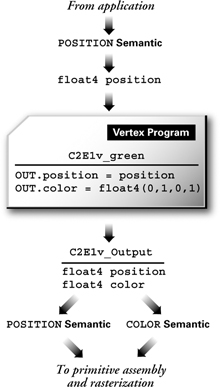
\includegraphics[width=0.5\linewidth]{Images/fig2_1.jpg}
    \caption{The Flow of Semantic Inputs and Outputs for \textbf{C2E1v\_green}}
    \label{fig:2-1}
\end{figure}

Input and output semantics are not the same, even though some have the same names. For example, for an input parameter to a vertex program, \textbf{POSITION} refers to the application-specified position assigned by the application when it sends a vertex to the GPU. However, an output structure element with the \textbf{POSITION} semantic represents the clip-space position that is fed to the hardware rasterizer.

Both semantics are named \textbf{POSITION} and, indeed, each is a position. However, each position semantic refers to a position at different points along the graphics pipeline. Your Cg vertex program transforms the application-supplied vertex position into a vertex suited for primitive assembly, clipping, and rasterization. In the \textbf{C2E1v\_green} program, this transformation is trivial (the vertex position is passed along unchanged), but later in this book, particularly in Chapters 4 and 5, you will learn more useful and interesting ways to transform vertices.

\subsection{The Function Body}

The substance of the \textbf{C2E1v\_green} function is contained in its body:

\FloatBarrier
\begin{lstlisting}
{
  C2E1v_Output OUT;
  OUT.position = float4(position, 0, 1);
  OUT.color    = float4(0, 1, 0, 1);  // RGBA green
  return OUT;
}
\end{lstlisting}
\FloatBarrier

Because the function's return type is \textbf{C2E1v\_Output}, you must declare a variable of this type to hold the value that the function returns. We often call a structure returned by an entry function an \textit{output structure}. The function body sets both elements of this structure variable and returns the structure. (Note that the entry function's return type is not required to have the same prefix as the entry function, although we've chosen to make them the same in our examples.)

The dot between \textbf{OUT} and \textbf{position}, as well as \textbf{OUT} and \textbf{color}, is the \textit{member operator} and gives access to a member within a structure. This is the same way that C and C++ access structure members. Think of a structure as a container for multiple values. The member operator lets you retrieve the values contained in a structure:

\FloatBarrier
\begin{lstlisting}
   OUT.position = float4(position, 0, 1);
   OUT.color    = float4(0, 1, 0, 1); // RGBA green
\end{lstlisting}
\FloatBarrier

First, the program assigns the \textbf{position} input parameter to \textbf{OUT.position}. However, the output structure member \textbf{OUT.position} is of type \textbf{float4} (Chapter 4 explains why). The expression \textbf{float4 (position, 0, 1)} converts a two-component position vector to a four-component vector by setting the third and fourth components to 0 and 1, respectively.

Second, the program assigns the RGBA color value for green to \textbf{OUT.color}. To provide the numeric value for green, construct the appropriate four-component color vector. The type of the \textbf{color} member is \textbf{float4} because the color is an RGBA color. The "A" in RGBA stands for "alpha," which normally encodes a measure of how opaque or transparent a color value is. The value 1 for alpha means the color is fully opaque.

When you use the \textbf{float4} or similar vector type name like a function (for example, \textbf{float4(0, 1, 0, 1)}), this is a called a \textit{constructor}. This constructor creates a value of the type specified out of the values listed in the parentheses. C++ has the concept of constructors, but C does not. Constructors in Cg are provided for vectors and matrices.

The syntax \textbf{float4(0, 1, 0, 1)} creates a vector <0, 1, 0, 1> that is assigned to the \textbf{color} member of type \textbf{float4} in \textbf{OUT}. The vector <0, 1, 0, 1> is green because the color components are in the red, green, blue, alpha (RGBA) order with a green (and alpha) contribution specified, but no red or blue contribution.

\FloatBarrier
\begin{lstlisting}
    return OUT;
\end{lstlisting}
\FloatBarrier

Finally, the \textbf{return} statement returns the output structure you initialized. The collection of values within \textbf{OUT} is passed along to the next stage of the graphics pipeline, as indicated by the semantics assigned to each member.

\section{Compiling Your Example}

You use the Cg runtime to load and compile Cg programs. When you compile a program, you must specify two things in addition to the text of the program:

\FloatBarrier
\begin{itemize}
\item The name of the entry function to compile
\item The profile name for the entry function to compile
\end{itemize}
\FloatBarrier

The name of the entry function in Example 2-1 is \textbf{C2E1v\_green} .

\textbf{C2E1v\_green} is a vertex program, so you need to compile for a vertex profile. The vertex profile you choose depends on the programming interface your application uses for 3D rendering (OpenGL or Direct3D), as well as the hardware capabilities of your GPU.

\subsection{Vertex Program Profiles}

There are several appropriate vertex profiles for compiling our example, as listed in Table \ref{table:2-1}. Future GPUs will no doubt support profiles that are more capable.

\begin{table}
\centering
\begin{tabular}{ |c|c|c|c|c|c|c|c| } 
 \hline
Profile Name & Programming Interface & Description \\
arbvp1 & OpenGL & Basic multivendor vertex programmability (corresponding to ARB\_vertex\_program functionality) \\
vs\_1\_1 & DirectX 8 & Basic multivendor vertex programmability \\
vp20 & OpenGL & Basic NVIDIA vertex programmability (corresponding to NV\_vertex\_program functionality) \\
vs\_2\_0 vs\_2\_x & DirectX 9 & Advanced multivendor vertex programmability \\
vp30 & OpenGL & Advanced NVIDIA vertex programmability (corresponding to NV\_vertex\_program2 functionality) \\
 \hline
\end{tabular}
\caption{Cg Vertex Profiles}
\label{table:2-1}
\end{table}

Your first example is very simple, so there is no problem compiling it with any of the profiles in Table 2-1, or any future vertex profile for that matter. As you progress through the book, you'll encounter some complex Cg programs that will require advanced vertex or fragment profiles. When an advanced profile is required, we are careful to point that out. Most examples in this book are written to compile for a broad range of Cg profiles.

Because you'll want your \textbf{C2E1v\_green} example to compile on the broadest range of GPUs, the best profiles for your example are \textbf{arbvp1} for OpenGL and \textbf{vs\_1\_1} for DirectX 8. Is there any reason to choose another profile? Yes, if you want to use advanced vertex programmability functionality, such as complex flow control or fast hardware instructions, which are not available in the basic profiles. For example, if you choose the \textbf{vp30} profile, you can write a Cg vertex program that loops a varying (nonconstant) number of times.

\subsection*{Coding Tip}

If there is a basic profile that is sufficient for compiling your Cg example, use it to gain the broadest hardware support. However, if you choose a more advanced profile, your Cg program may execute more efficiently and you can program using more general programming practices.
\hrule

So what is the disadvantage of a more advanced profile? It may limit your program to newer GPUs. To get the best of both worlds—broad hardware support as well as the latest available hardware—you might provide both a fallback Cg program for basic profiles and a more advanced Cg program for more advanced profiles. The CgFX format simplifies this approach by providing a unified way to encapsulate multiple Cg implementations of a given rendering effect in a single source file. Appendix C explains more about CgFX.

Refer to Appendix B to learn how an application can use the Cg runtime library to load and compile Cg programs. In general, you call a set of Cg runtime routines that require your program text, your entry function name, and your chosen profile. If there are errors in your program, the compilation will fail. You can request a list of compile errors to assist you in correcting your code. Once your program compiles successfully, other Cg runtime routines assist you in configuring your 3D programming interface of choice (OpenGL or Direct3D) to render with your program.

\subsection{Classes of Cg Compilation Errors}

There are two classes of compilation errors for Cg programs: conventional and profile-dependent.

\textit{Conventional errors} are caused either by incorrect syntax, usually due to typos, or by incorrect semantics, such as calling a function with the wrong number of parameters.

These types of errors are not fundamentally different from the everyday compile errors that C and C++ programmers deal with.

\textit{Profile-dependent errors} result from using Cg in a way that is syntactically and semantically correct but not supported by your specified profile. You may have written valid Cg code, but it might not compile because of the profile you specified. General-purpose programming languages do not have this type of error.

\subsection{Profile-Dependent Errors}

Profile-dependent errors are usually caused by limitations of the 3D programming interface and the underlying GPU hardware for which you are attempting to compile your program. There are three categories of profile-dependent errors: capability, context, and capacity.

\subsection*{Capability}

All current profiles for fragment programs permit texture accesses, but no current vertex profiles do. The reason for this is simple. The programmable vertex processors in most current GPUs do not support texture accesses. Future vertex profiles are likely to permit texture accesses.

Cg does not allow you to compile a program that is impossible to execute, given the specified profile for compilation. If a vertex profile does not support texture accesses, a profile-dependent error of capability occurs. The hardware, or the 3D programming interface, lacks the ability to do what Cg allows you to express.

\subsection*{Context}

An error of profile-dependent context is more fundamental, though rare. For example, it is an error to write a vertex program that does not return exactly one parameter that is bound to the \textbf{POSITION} semantic. This is because the remainder of the graphics pipeline assumes that all vertices have a position.

Likewise, a fragment profile cannot return a \textbf{POSITION} the way a vertex profile must. Such errors are caused by using Cg in a manner inconsistent with the data flow of the graphics pipeline.

\subsection*{Capacity}

Capacity errors stem from a limit on a GPU's capability. Some GPUs can perform only four texture accesses in a single rendering pass. Other GPUs can perform any number of texture accesses in a single rendering pass, restricted only by the number of fragment program instructions the hardware supports. If you access more than four textures in a profile that does not permit access to more than four textures, you receive a capacity error.

Capacity errors are probably the most frustrating, because it may not be apparent from looking at your program what the exceeded capacity is. For example, you may have exceeded the maximum number of vertex program instructions allowed by the GPU in a single program, but that fact may not be obvious.

\subsection*{Preventing Errors}

There are two ways to avoid these frustrating errors. One is to use a more advanced profile. The more advanced a profile is, the less chance you have of bumping into the capability and capacity limits of the profile. As the functionality of programmable graphics hardware improves, you will worry less and less about capability and capacity limits.

Another solution is to educate yourself about the limitations of capability, context, and capacity for the profiles you use in your 3D application. Consult the documentation that accompanies the Cg Toolkit to learn about these limits.

You can often get a good sense of the profile-dependent restrictions by knowing the limitations of the raw 3D programming interface you are using. Consult your OpenGL and Direct3D documentation; it will help you identify Cg constructs that might be subject to profile-dependent limitations.

\subsection{The Norm: Multiple Entry Functions}

C and C++ programs begin executing when the operating system invokes a program instance and calls the program's \textbf{main} routine (or \textbf{WinMain} routine for Windows programs). Example 2-1 is complete, but it has no routine named \textbf{main}. Why? Because, instead, we named the entry function \textbf{C2E1v\_green} . In this book, we adhere to our naming convention to distinguish our examples from each other and to make them easy to locate. In your own 3D application, however, you can name the entry function whatever you choose, as long as the name is a valid identifier.

Your 3D application will typically use a collection of Cg programs, not just one. At a minimum, you will probably have one vertex program and one fragment program, though you can use the fixed-function pipeline for vertex processing, fragment processing, or even both if you wish. A complex application may have hundreds of Cg programs. Because Cg programs can be compiled at runtime, you can even generate new Cg programs while your application is running, by formatting Cg program text procedurally.

Of course, you can still use the name \textbf{main}, which is the default entry function name for Cg programs if no explicit entry function name is specified when you compile Cg source code.

\subsection*{Coding Tip}

To avoid confusion, find descriptive names for your entry functions. If all your entry functions are named \textbf{main}, it will be difficult to have several entry functions in a single Cg source file—even if that is the default entry function name assumed by the runtime.
\hrule

\subsection{Downloading and Configuring Vertex and Fragment Programs}

In a general-purpose language, the operating system invokes the \textbf{main} (or \textbf{WinMain}) routine and the program executes the code contained in that \textbf{main} routine. If the \textbf{main} routine returns, the program terminates.

However, in Cg, you do not invoke a program that runs until it terminates, as you would in C or C++. Instead, the Cg compiler translates your program into a form that your 3D programming interface can download to hardware. It is up to your application to call the necessary Cg runtime and 3D programming interface routines to download and configure your program for use by the GPU.

Figure \ref{fig:2-2} shows how an application compiles a Cg program and converts it into a binary microcode that the GPU's vertex processor directly executes when transforming vertices.

\begin{figure}
    \centering
    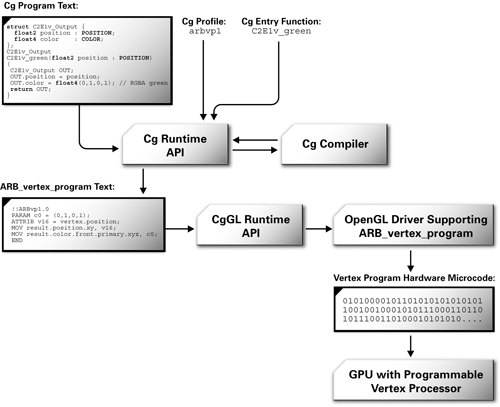
\includegraphics[width=1\linewidth]{Images/fig2_2.jpg}
    \caption{Compiling and Loading a Cg Program into the GPU}
    \label{fig:2-2}
\end{figure}

Once loaded with a vertex program, the programmable vertex processor in your GPU runs that program every time the application feeds a vertex to the GPU. When it renders a complex model with thousands of vertices, your current vertex program processes every vertex in the model. The vertex program runs once for each vertex.

A single current vertex program is loaded in the programmable vertex processor for execution at any one time. However, your application may change the current vertex program, as needed.

This same concept of a single current program applies to the programmable fragment processor in your GPU too. You compile your Cg fragment program and use the Cg runtime, along with your 3D programming interface, to download your program and bind it as the current fragment program for processing fragments generated by the rasterizer. After your fragment program is bound, 3D primitives are rasterized into fragments and your current fragment program processes each generated fragment. The fragment program runs once for each fragment.

Typically, 3D applications co-program the programmable vertex and fragment processors in the GPU to achieve a particular rendering effect. This approach is very efficient because of the parallel and highly pipelined nature of the programmable vertex and fragment processors in GPUs.

\section{A Simple Fragment Program}

So far, our example involves only a vertex program, \textbf{C2E1v\_green}. This section presents a simple fragment program that you can use with our vertex program.

Example 2-2 shows the complete Cg source code for our first fragment program.

\FloatBarrier
\begin{lstlisting}[caption=Example 2-2. The \textbf{C2E2f\_passthrough} Fragment Program]
struct C2E2f_Output {
  float4 color : COLOR;
};

C2E2f_Output C2E2f_passthrough(float4 color : COLOR)
{
  C2E2f_Output OUT;
  OUT.color = color;
  return OUT;
}
\end{lstlisting}
\FloatBarrier

This program is even simpler than the example for the \textbf{C2E1v\_green} vertex program. In fact, it does almost nothing. The program outputs the unchanged interpolated color assigned for every fragment generated by the rasterizer. The GPU's raster operation hardware uses this color to update the frame buffer if the fragment survives the various raster operations, such as scissoring and depth testing.

Here is the output structure returned by \textbf{C2E2f\_passthrough}:

\FloatBarrier
\begin{lstlisting}
struct C2E2f_Output {
  float4 color : COLOR;
};
\end{lstlisting}
\FloatBarrier

Fragment programs have a simpler output structure than vertex programs. A vertex program must output a position and may return one or more colors, texture coordinate sets, and other per-vertex outputs. A fragment program, however, must reduce everything to a single color that will update the frame buffer. (In some advanced profiles, fragment programs can write additional data such as a depth value as well.) The \textbf{COLOR} semantic assigned to the \textbf{color} member in a fragment program indicates that the member is the color to be used to update the frame buffer.

The entry function declaration for \textbf{C2E2f\_passthrough} is this:

\FloatBarrier
\begin{lstlisting}
C2E2f_Output C2E2f_passthrough(float4 color : COLOR)
\end{lstlisting}
\FloatBarrier

The function returns the \textbf{C2E2f\_Output} output structure with one color. The function receives a single four-component vector, named "color," bound to the \textbf{COLOR} input semantic. The \textbf{COLOR} input semantic for a fragment program is the color of the fragment interpolated by the rasterizer, based on the primitive's assigned vertex colors.

The body of \textbf{C2E2f\_passthrough} is this:

\FloatBarrier
\begin{lstlisting}
{
  C2E2f_Output OUT;
  OUT.color = color;
  return OUT;
}
\end{lstlisting}
\FloatBarrier

After declaring an \textbf{OUT} variable with the \textbf{C2E2f\_Output} output structure type, the program assigns the fragment's interpolated color (the single input parameter) to the final fragment color in the output structure. Finally, the program returns the \textbf{OUT} structure.

\subsection{Fragment Program Profiles}

Just as you needed a profile to compile the \textbf{C2E1v\_green} example, you also need a profile to compile the \textbf{C2E2f\_passthrough} example. However, the profiles for compiling the \textbf{C2E1v\_green} example were for vertex programs. To compile \textbf{C2E2f\_passthrough} , you must choose an appropriate fragment profile.

Table \ref{table:2-2} lists various profiles for compiling fragment programs.

\begin{table}
\centering
\begin{tabular}{ |c|c|c|c|c|c|c|c| } 
 \hline
Profile Name & Programming Interface & Description \\
ps\_1\_1 ps\_1\_2 ps\_1\_3 & DirectX 8 & Basic multivendor fragment programmability \\
fp20 & OpenGL & Basic NVIDIA fragment programmability (corresponding to NV\_texture\_shader and NV\_register\_combiners functionality) \\
arbfp1 & OpenGL & Advanced multivendor fragment programmability (corresponding to ARB\_fragment\_program functionality) \\
ps\_2\_0 ps\_2\_x & DirectX 9 & Advanced multivendor fragment programmability \\
fp30 & OpenGL & Advanced NVIDIA fragment programmability (corresponding to NV\_fragment\_program functionality) \\
 \hline
\end{tabular}
\caption{Cg Fragment Profiles}
\label{table:2-2}
\end{table}

Like the earlier vertex program example, this first fragment program example is so simple that you can compile the \textbf{C2E2f\_passthrough} example with any of the profiles in Table \ref{table:2-2}.

Cg has a command-line compiler known as \textbf{cgc}, which is short for "Cg compiler." Dynamic compilation at runtime can be very powerful and is highly recommended. However, when you are writing Cg programs, you often want to verify that they compile correctly without having to run your 3D application. To detect Cg compiler errors while writing programs, try running \textbf{cgc}. It will "test compile" the Cg program files used by your application as part of your regular application build process. Using \textbf{cgc} in an integrated development environment (IDE) such as Microsoft's Visual C++ can make it quick and easy to find compilation errors. A good IDE will even help you quickly locate the appropriate line of code, based on line numbers in the error message, just as you would with C or C++ programs. Figure \ref{fig:2-3} shows an example of debugging compiler errors in Microsoft Visual Studio.

\begin{figure}
    \centering
    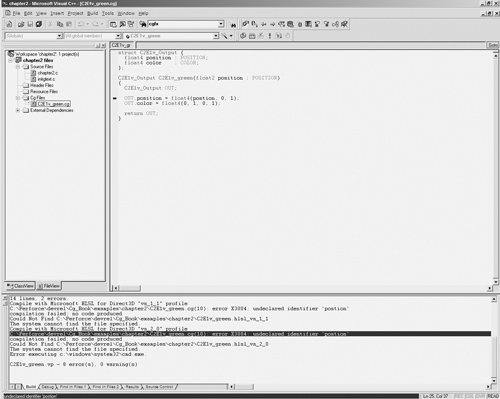
\includegraphics[width=1\linewidth]{Images/fig2_3.jpg}
    \caption{Locating Error Lines in an Integrated Development Environment}
    \label{fig:2-3}
\end{figure}

\subsection*{Coding Tip}

Cg developers often write a single Cg program that works for both OpenGL and Direct3D, even if they predominantly use one programming interface or the other. However, profile-dependent differences can exist between what is valid in the corresponding profiles for these 3D programming interfaces. So make it your practice to compile your Cg programs twice with \textbf{cgc}: once for the appropriate OpenGL profile, and again for the appropriate Direct3D profile.
\hrule

\section{Rendering with Your Vertex and Fragment Program Examples}

Now it's time to see your two simple Cg programs in action. Don't expect too much, because these are both very simple programs. However, you can still learn a lot by examining how the programs work together—and with the rest of the graphics pipeline—to draw a green triangle.

Look at the 2D triangle in Figure \ref{fig:2-4}. This is the geometry that your vertex and fragment program will operate on in this example.

\begin{figure}
    \centering
    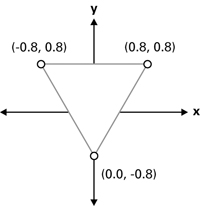
\includegraphics[width=0.5\linewidth]{Images/fig2_4.jpg}
    \caption{A 2D Triangle for Rendering}
    \label{fig:2-4}
\end{figure}

\subsection{Rendering a Triangle with OpenGL}

In OpenGL, you can render this 2D triangle with the following commands:

\FloatBarrier
\begin{lstlisting}
glBegin(GL_TRIANGLES);
  glVertex2f(-0.8, 0.8);
  glVertex2f(0.8, 0.8);
  glVertex2f(0.0, -0.8);
glEnd();
\end{lstlisting}
\FloatBarrier

\subsection{Rendering a Triangle with Direct3D}

In Direct3D, you can render the same triangle with the following code:

\FloatBarrier
\begin{lstlisting}
D3DXVECTOR4 vertices[3] =
{
    D3DXVECTOR4(-0.8f,  0.8f, 0.f, 1.f),
    D3DXVECTOR4( 0.8f,  0.8f, 0.f, 1.f),
    D3DXVECTOR4( 0.0f, -0.8f, 0.f, 1.f),
};

m_pD3DDevice->DrawPrimitiveUP(D3DPT_TRIANGLELIST, 1,
  vertices, sizeof(D3DXVECTOR4));
\end{lstlisting}
\FloatBarrier

There are other, more efficient ways to transfer vertices to the GPU in OpenGL or Direct3D. When you use Cg programs to process vertices, it doesn't matter how the application sends the vertices to the GPU.

\subsection{Getting the Same Results}

Figure \ref{fig:2-5} shows the result of rendering this triangle with the \textbf{C2E1v\_green} vertex program and \textbf{C2E2f\_passthrough} fragment program configured. The result is the same, whether rendered with OpenGL or Direct3D. Admittedly, it's not very exciting, but the triangle is solid green.

\begin{figure}
    \centering
    
\includegraphics[width=0.25\linewidth]{Images/fig_0006.jpg}
    \caption{Rendering a Triangle with \textbf{C2E1v\_green} and \textbf{C2E2f\_passthrough}}
    \label{fig:2-5}
\end{figure}

The vertex program passes the specified 2D position of each vertex to the rasterizer. The rasterizer expects positions to be specified as coordinates in clip space. Clip space defines what is visible from the current viewpoint. If the vertex program supplies 2D coordinates, as is the case in Figure \ref{fig:2-5}, the portion of the primitive that is rasterized is the portion of the primitive where x and y are between -1 and +1. The entire triangle is within the clipping region, so the complete triangle is rasterized.

Figure \ref{fig:2-6} shows the region of rasterization for 2D clip space.

\begin{figure}
    \centering
    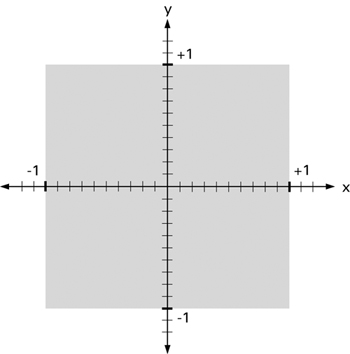
\includegraphics[width=0.5\linewidth]{Images/fig2_6.jpg}
    \caption{A 2D View of Clip Space}
    \label{fig:2-6}
\end{figure}

Primitives are rendered into the frame buffer if they fall within the gray region (the region of clip space where x and y are between -1 and +1). You'll learn more about clip space in Chapter 4.

Figure \ref{fig:2-7} shows what happens when you use the \textbf{C2E1v\_green} vertex program and \textbf{C2E2f\_passthrough} fragment program with 2D geometry that is not entirely within the visible region of 2D clip space. When the stars include vertices that have x or y coordinates outside the -1 to +1 region, the rasterizer clips some of the green stars by the edge of the visible region. If no part of a primitive is within the viewable region of clip space, the rasterizer eliminates the primitive.

\begin{figure}
    \centering
    
\includegraphics[width=0.25\linewidth]{Images/fig_0008.jpg}
    \caption{Primitives Rendered with and Require 2D Clipping}
    \label{fig:2-7}
\end{figure}

The GPU then transforms clip space automatically (by a simple scale and bias) into window space coordinates for the rasterizer. Effectively, the GPU stretches clip-space coordinates as necessary, prior to rasterization, to fit the rendering viewport and window position.

Chapter 4 generalizes this 2D notion of clip space to 3D, and includes perspective views. But in this chapter and Chapter 3, the examples use 2D rendering to keep things simple.

\section{Exercises}

\FloatBarrier
\begin{enumerate}
\item \textbf{Answer this:} What GPU profiles does your Cg compiler support? Consult your compiler's documentation or try running \textbf{cgc –help} at the command line. Which profiles are vertex profiles and which are fragment profiles?
\item \textbf{Try this yourself:} Modify the \textbf{C2E1v\_green} vertex program to color the vertices red instead of green.
\item \textbf{Try this yourself:} Change the one triangle vertex position by extending the vertex coordinates outside the [-1, +1] range. Run the example. Is the triangle clipped as you would expect?
\end{enumerate}
\FloatBarrier

\section{Further Reading}

Check out the documentation, such as the \textit{Cg Toolkit User's Manual: A Developer's Guide to Programmable Graphics}, that accompanies the Cg Toolkit software distribution.

Also, visit the Web site \textbf{www.cgshaders.org} for current Cg information. This site has articles, forums where you can ask questions, and freely available sample shader code.

\end{document}
